\documentclass[color=usenames,dvipsnames]{beamer}
%\documentclass[color=usenames,dvipsnames,handout]{beamer}

%\usepackage[roman]{../pres1}
\usepackage[sans]{../pres1}
\usepackage{graphicx}

\usepackage{color}




\begin{document}

\fboxsep=0mm

\begin{frame}[plain]
  \huge
  \begin{center}
    \huge Applied Population Dynamics \\
    \LARGE Lab 01 -- Excel Basics \\
    \large January 7 \& 11, 2019 \par
    \vspace{.5cm}
    \fbox{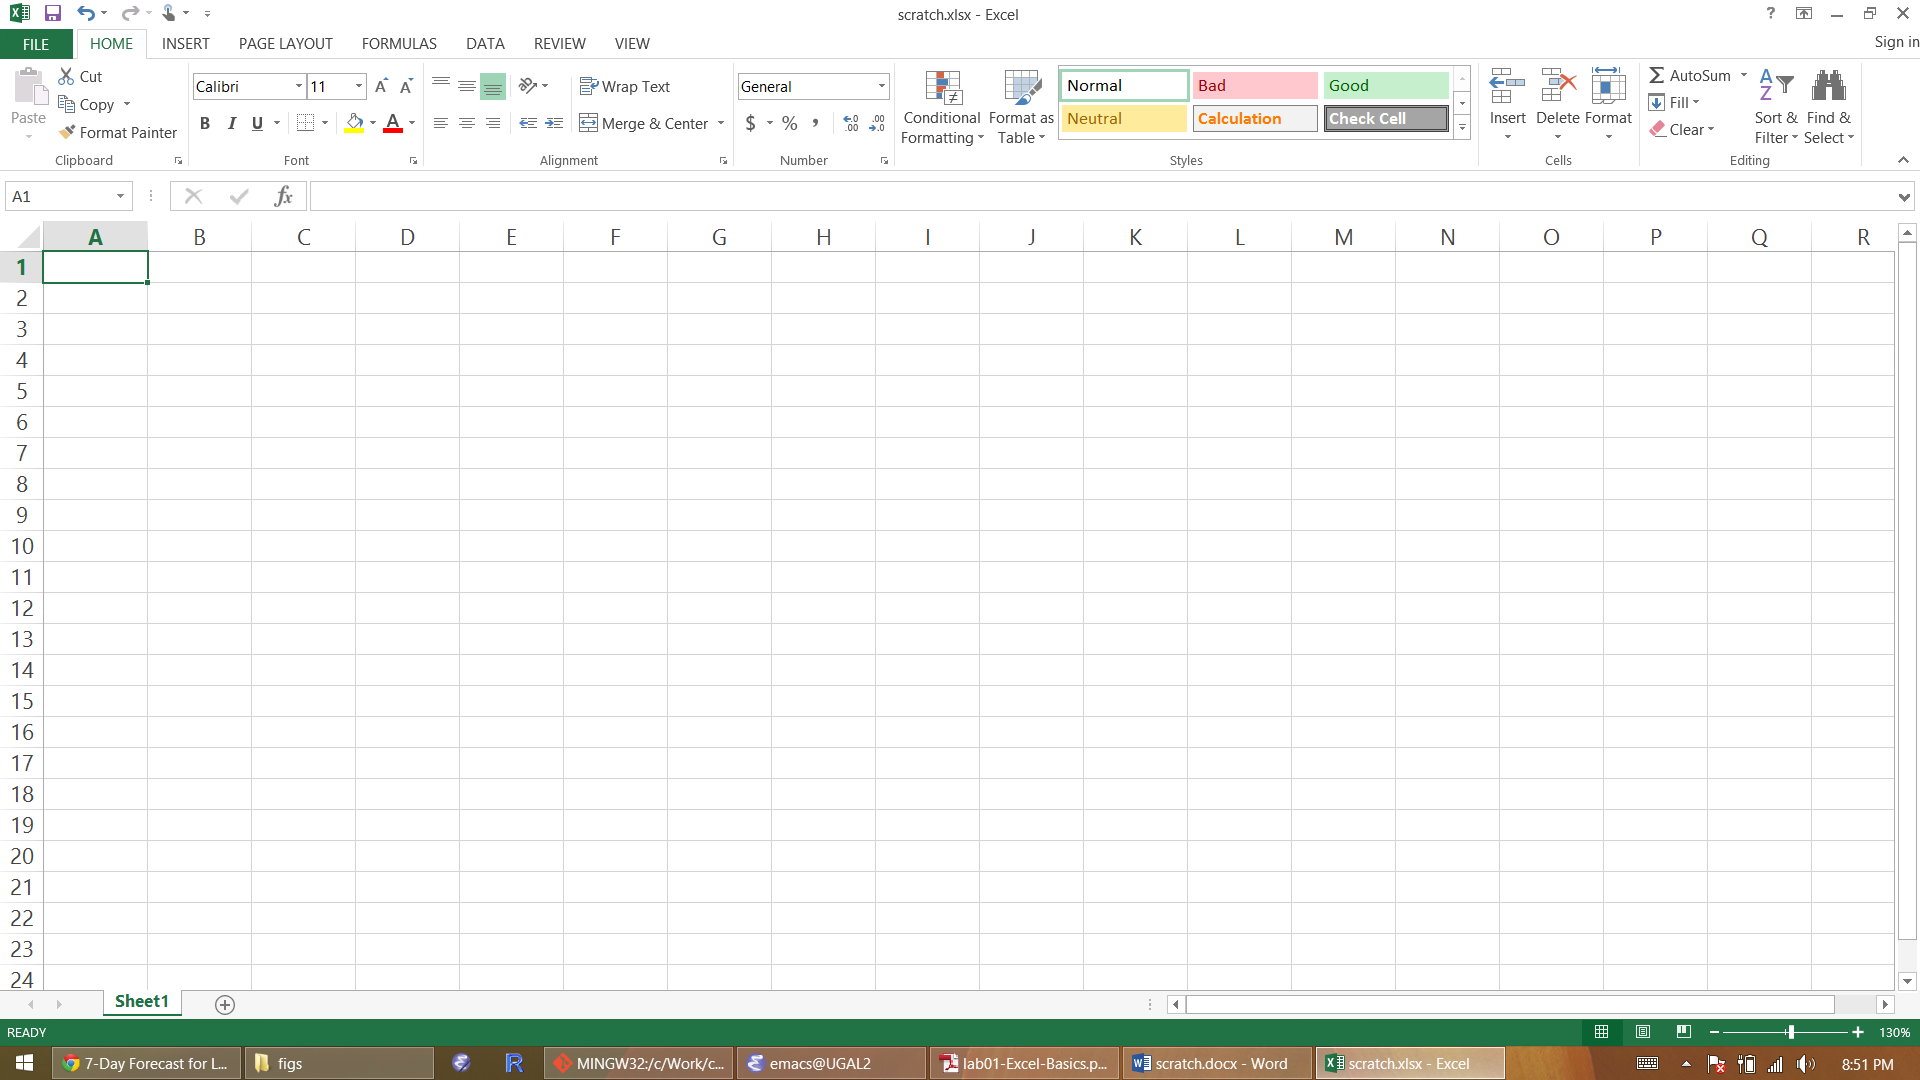
\includegraphics[width=\textwidth]{figs/excel}}
  \end{center}
%  \note{Describe structure... quick access toolbar, ribbon, sheets, workbooks, etc...}
\end{frame}


\section{Referencing}


\begin{frame}
  \frametitle{Column B}
  \fbox{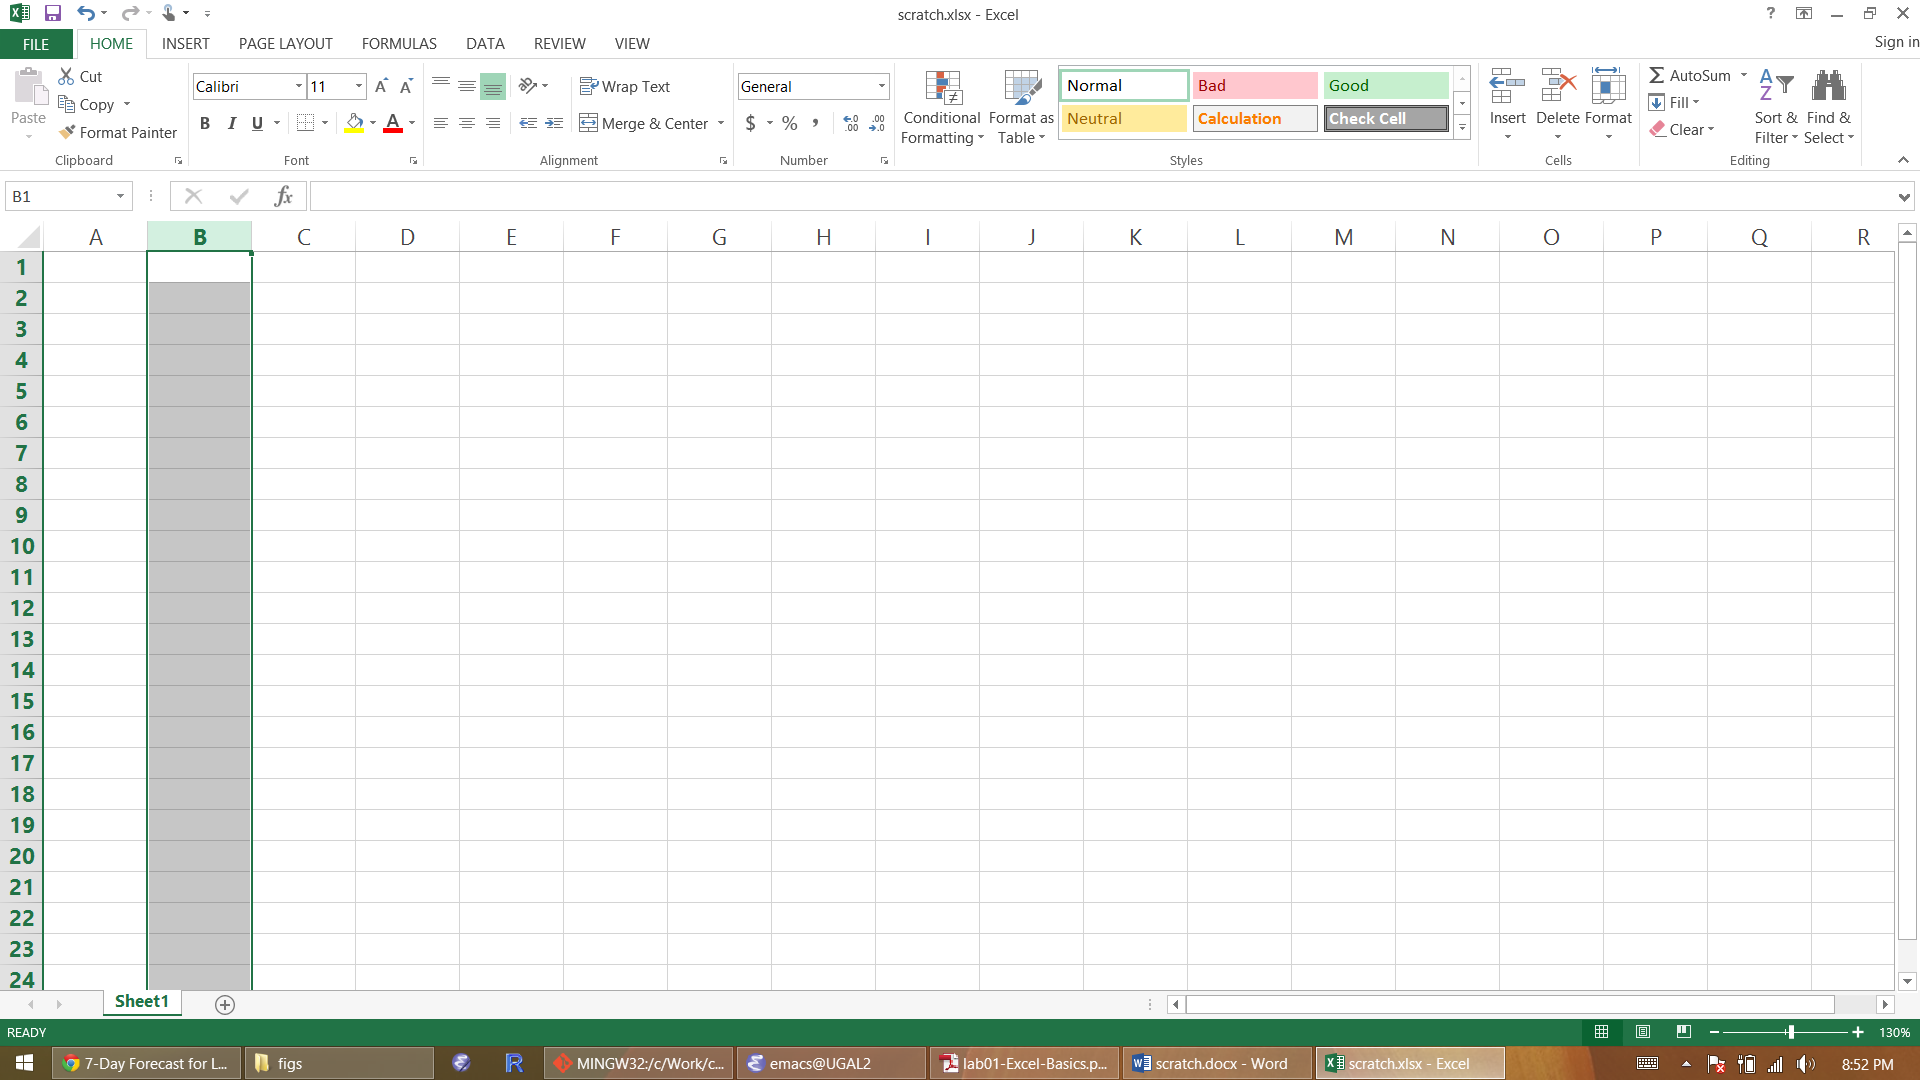
\includegraphics[width=\textwidth]{figs/columnB}}
\end{frame}


\begin{frame}
  \frametitle{Row 3}
  \fbox{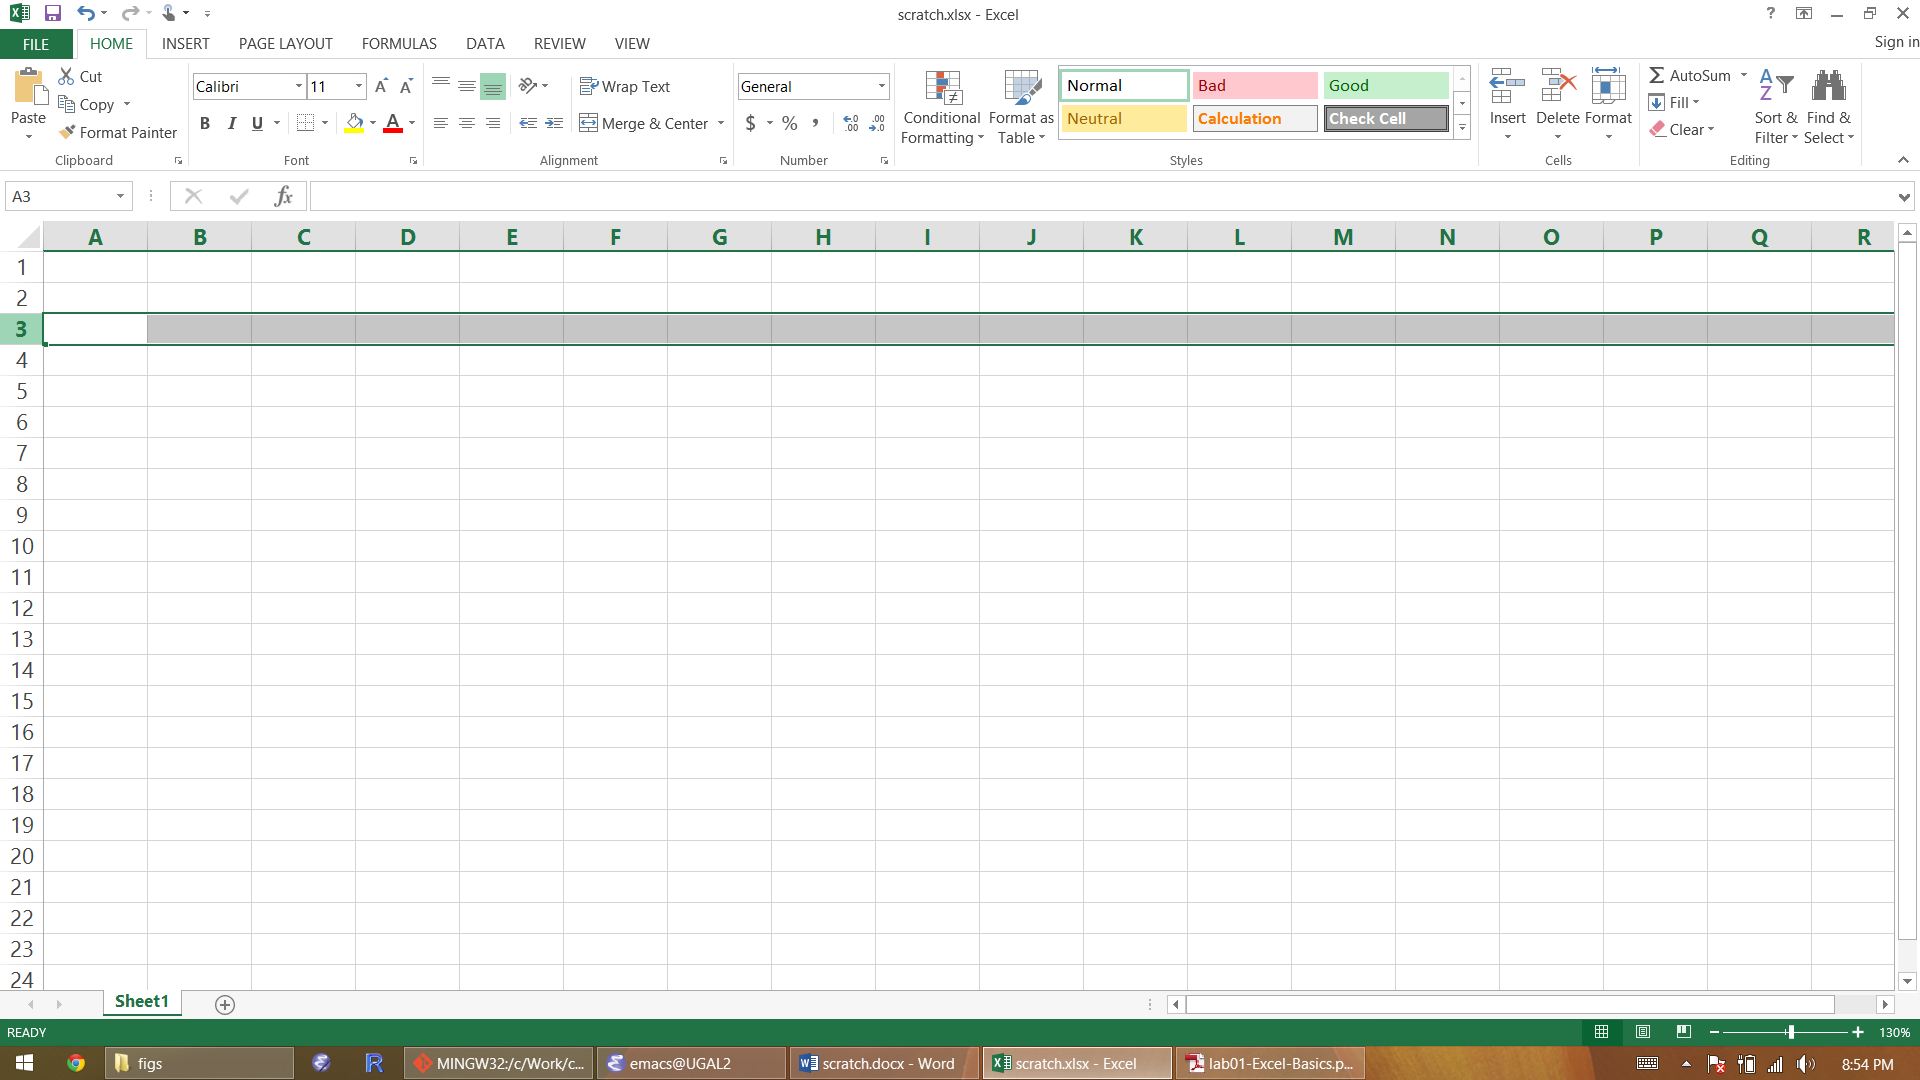
\includegraphics[width=\textwidth]{figs/row3}}
\end{frame}



\begin{frame}
  \frametitle{Cell B3}
  \fbox{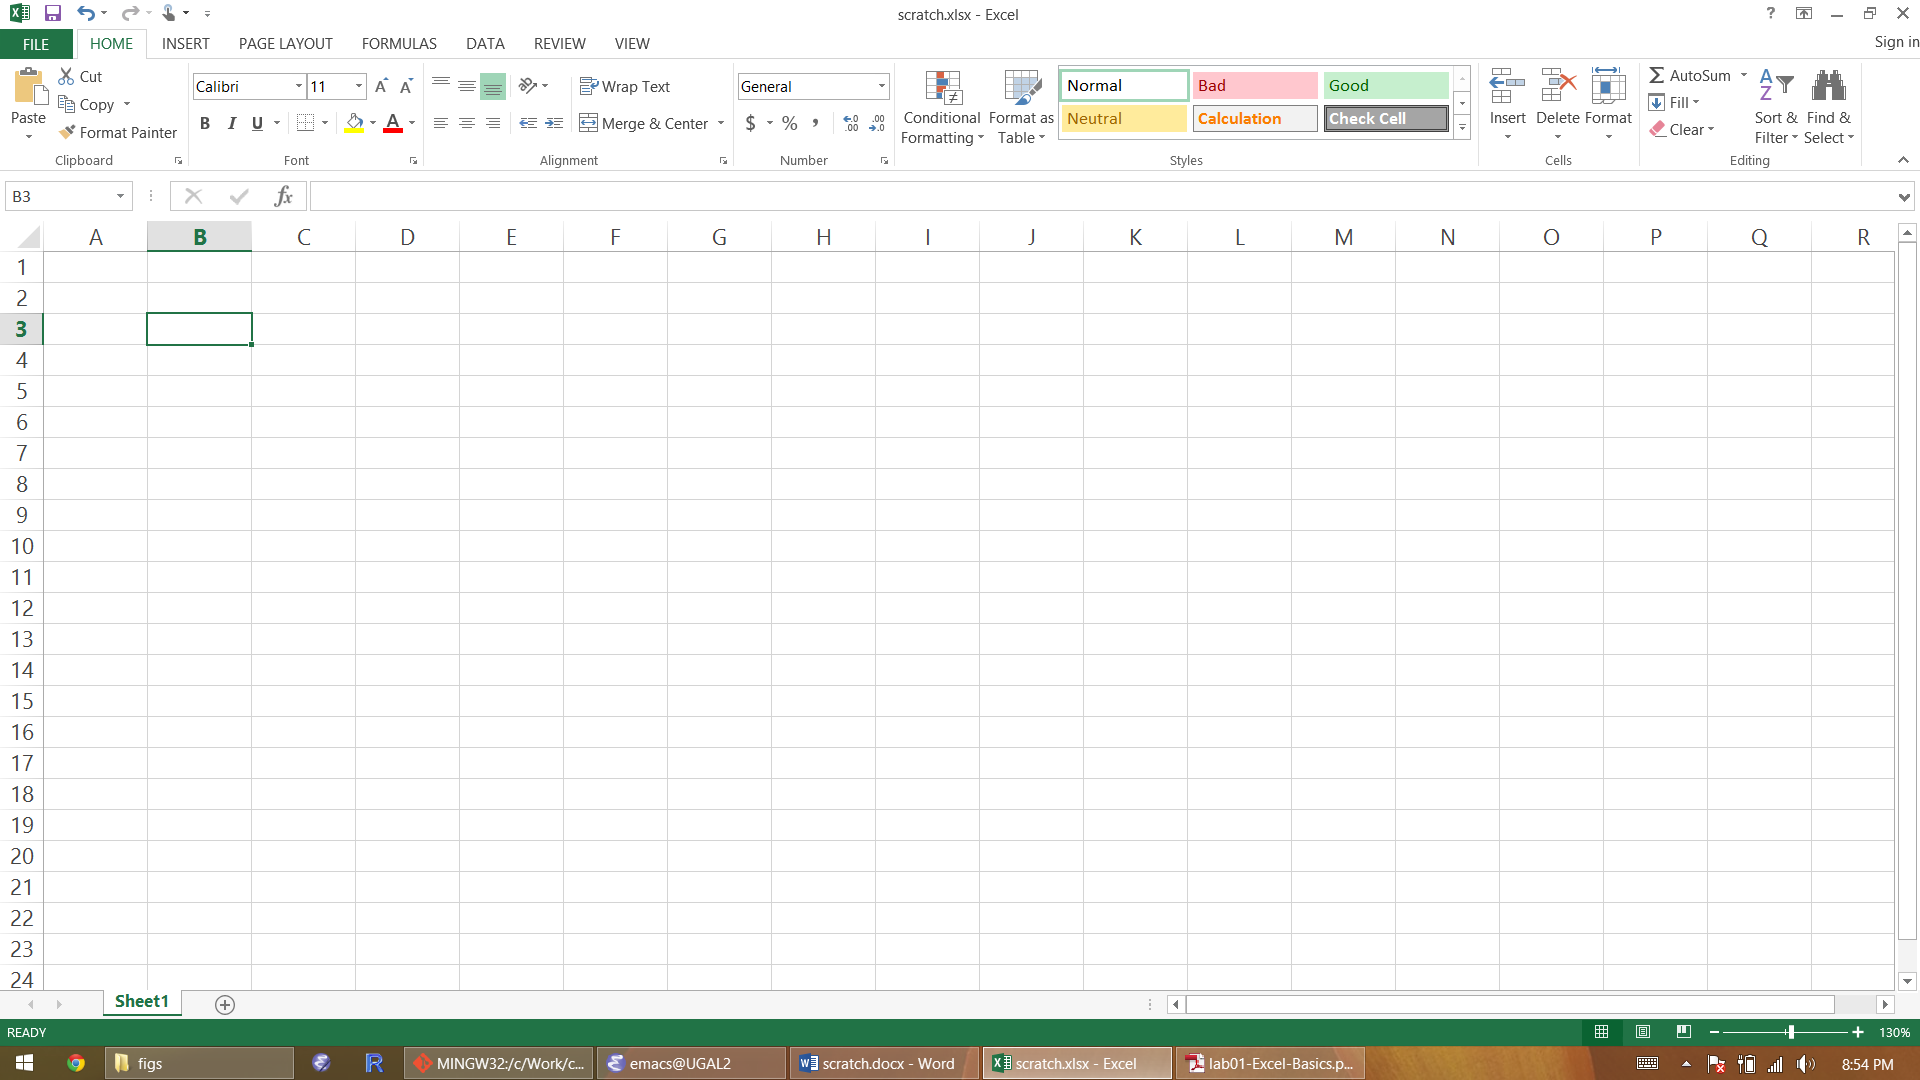
\includegraphics[width=\textwidth]{figs/cellB3}}
\end{frame}



\begin{frame}
  \frametitle{Create Sequence Using Auto-fill}
  \fbox{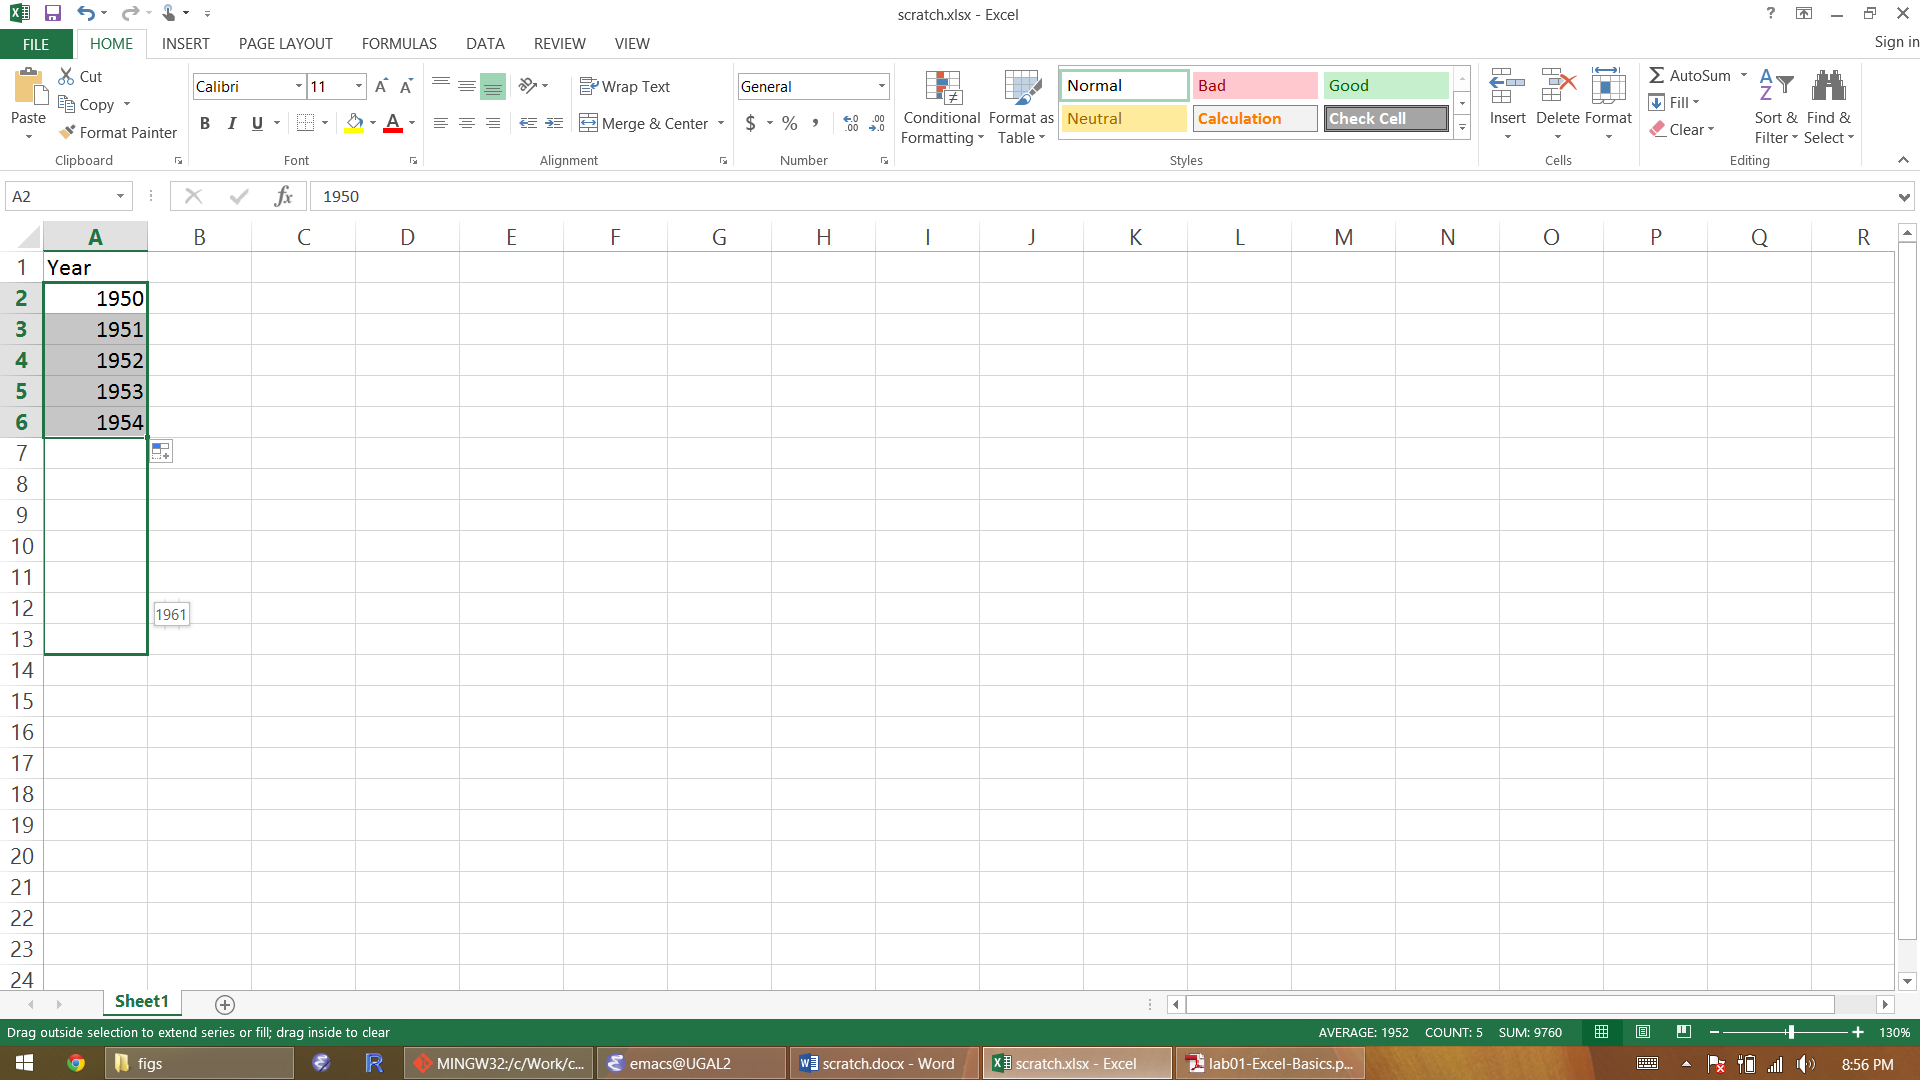
\includegraphics[width=\textwidth]{figs/sequence}}
\end{frame}


\begin{frame}
  \frametitle{Relative Cell References}
  \only<1>{\fbox{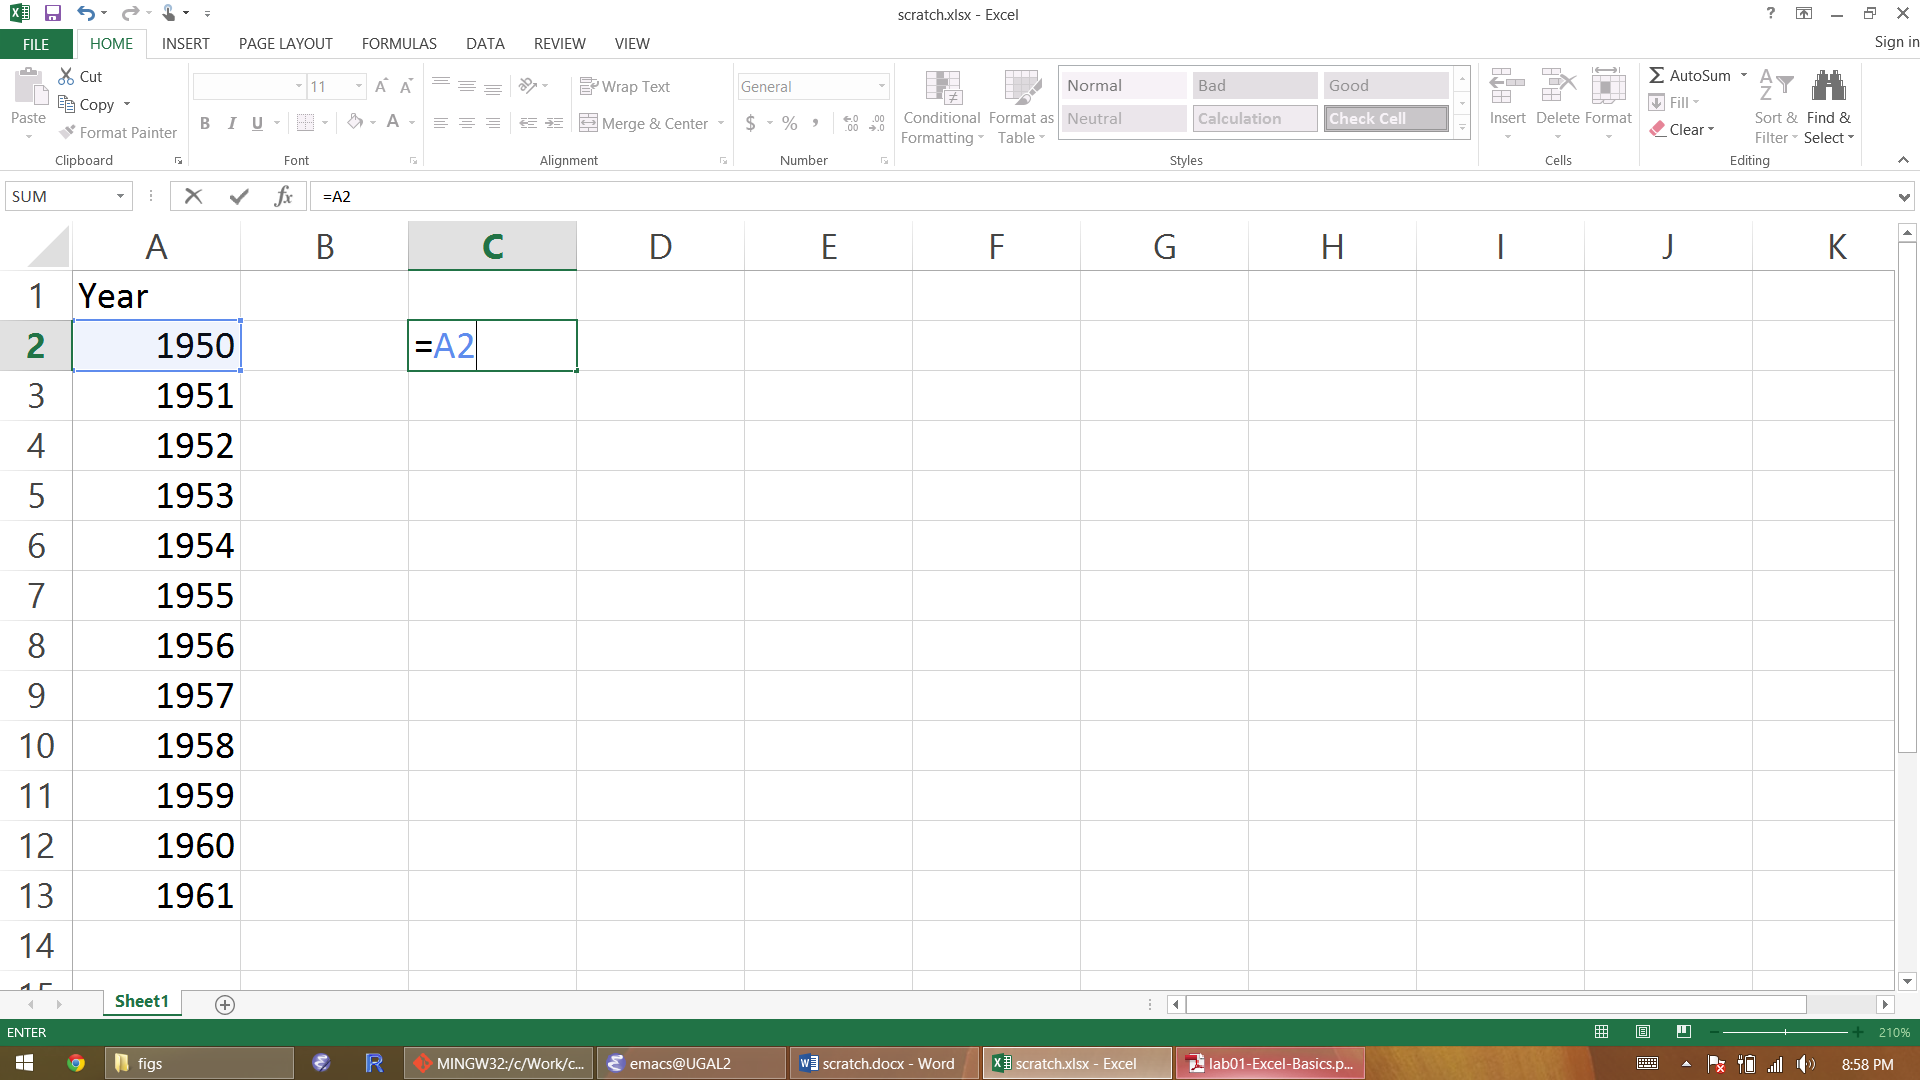
\includegraphics[width=\textwidth]{figs/relative-ref}}}
  \only<2 | handout:0>{\fbox{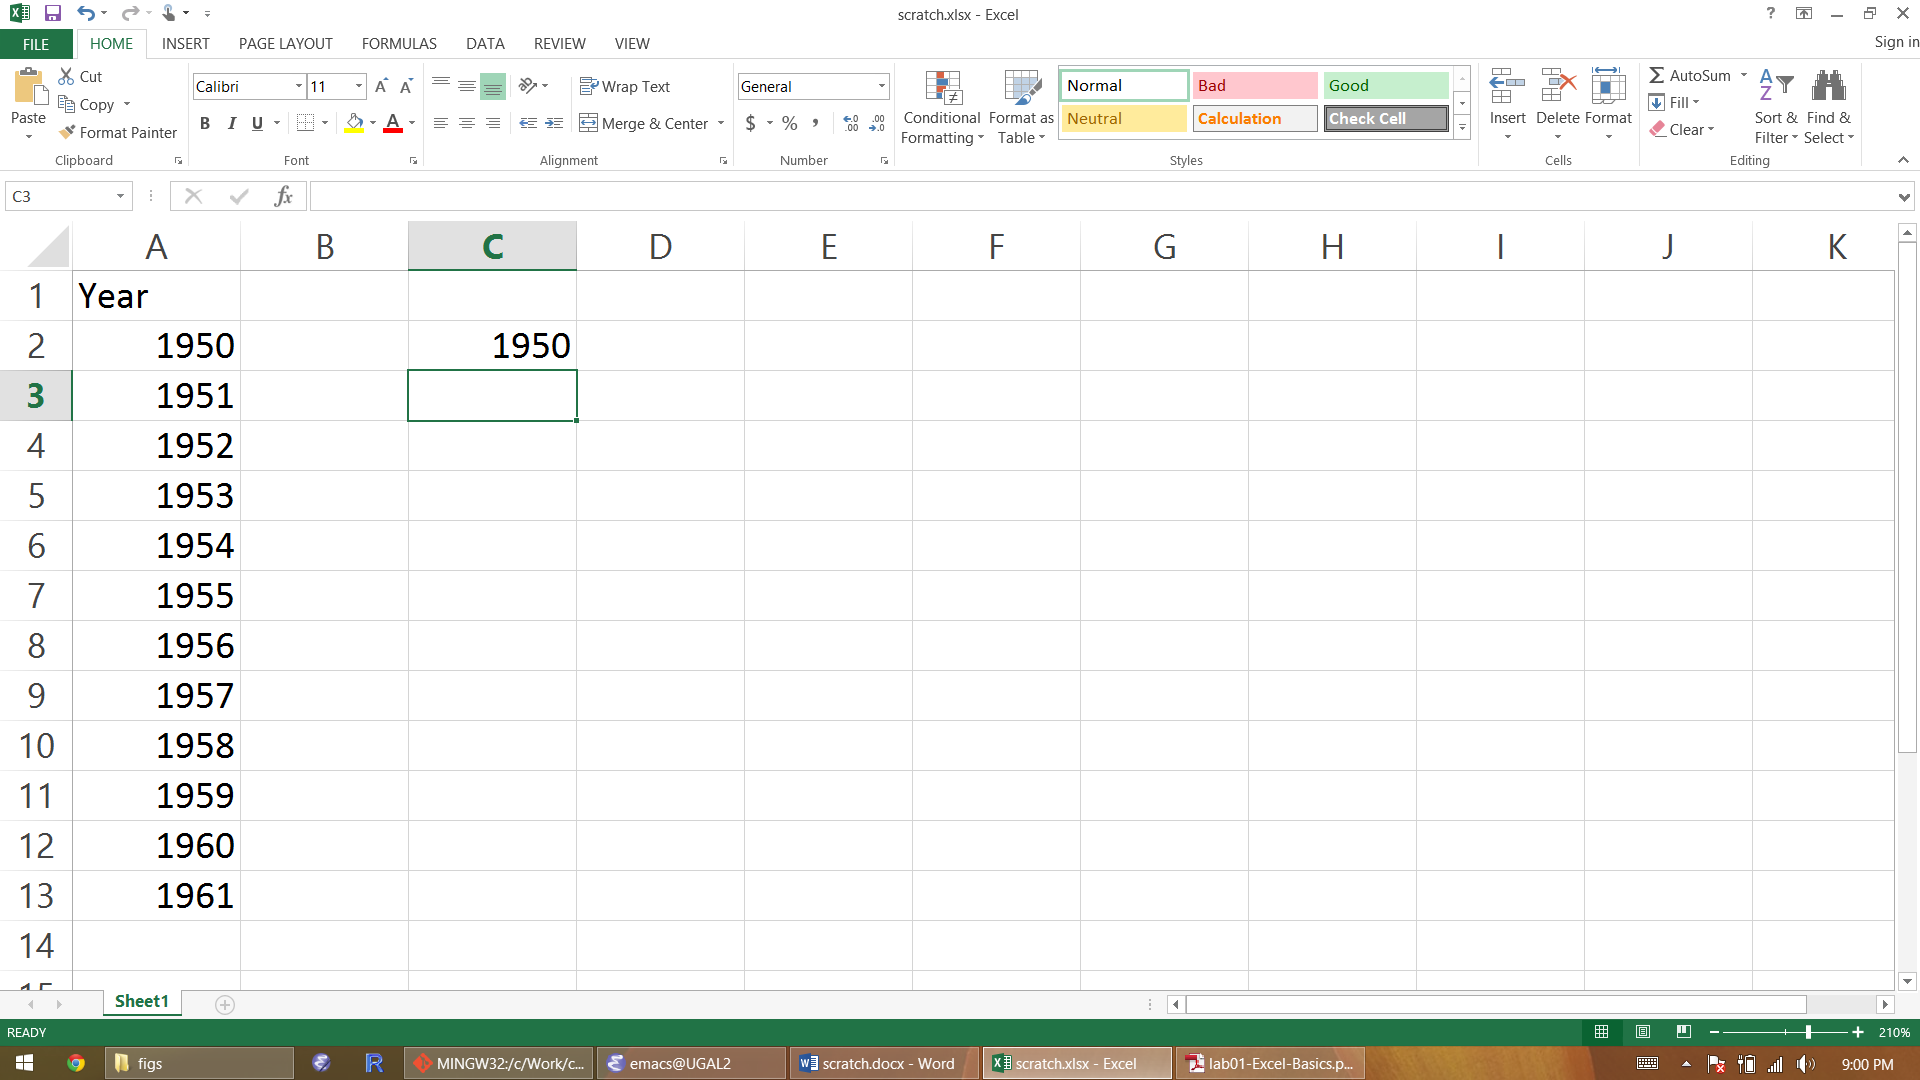
\includegraphics[width=\textwidth]{figs/relative-ref2}}}
  \begin{center}
    Cell C2 will take on the value of A2 \\
  \end{center}
\end{frame}


\begin{frame}
  \frametitle{Relative Cell References}
  \fbox{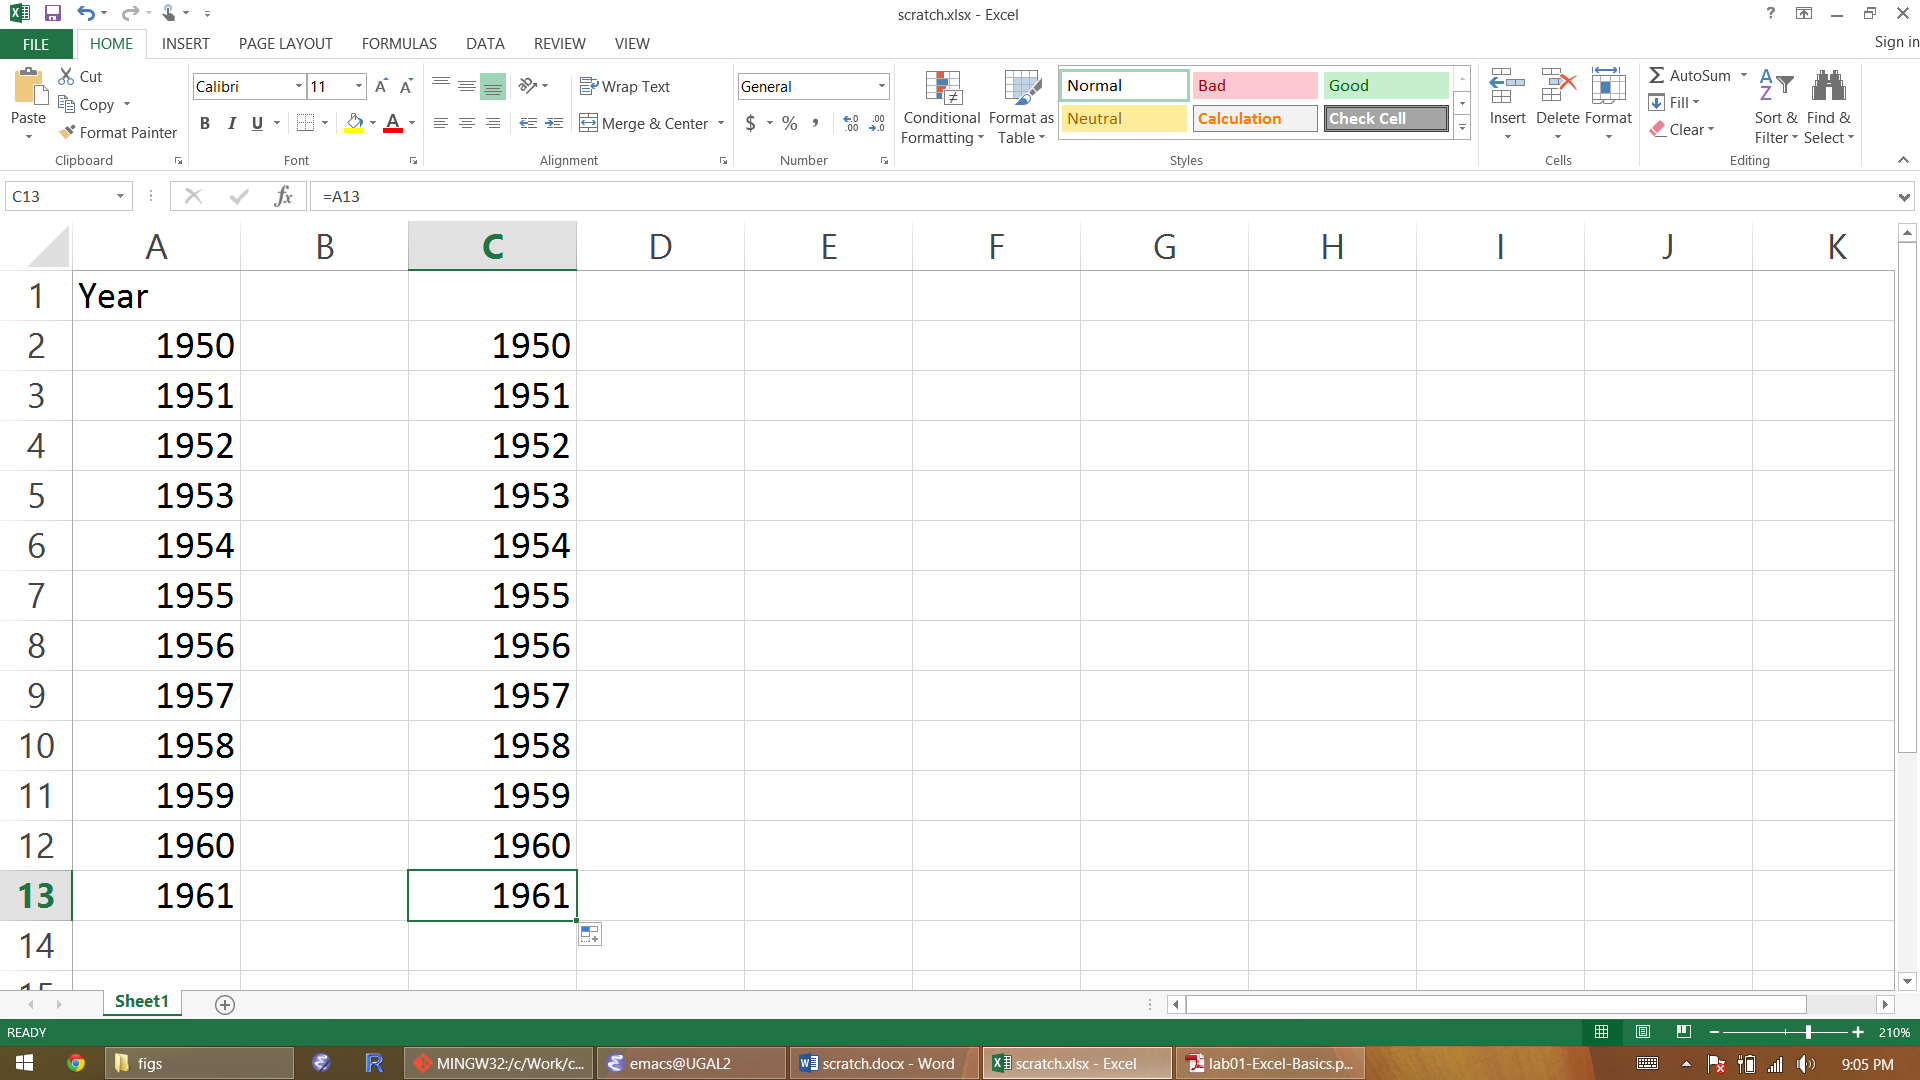
\includegraphics[width=\textwidth]{figs/relative-ref3}}
  \begin{center}
    Values of reference will change when using auto-fill
  \end{center}
\end{frame}


\begin{frame}
  \frametitle{Absolute Cell References}
  \only<1>{\fbox{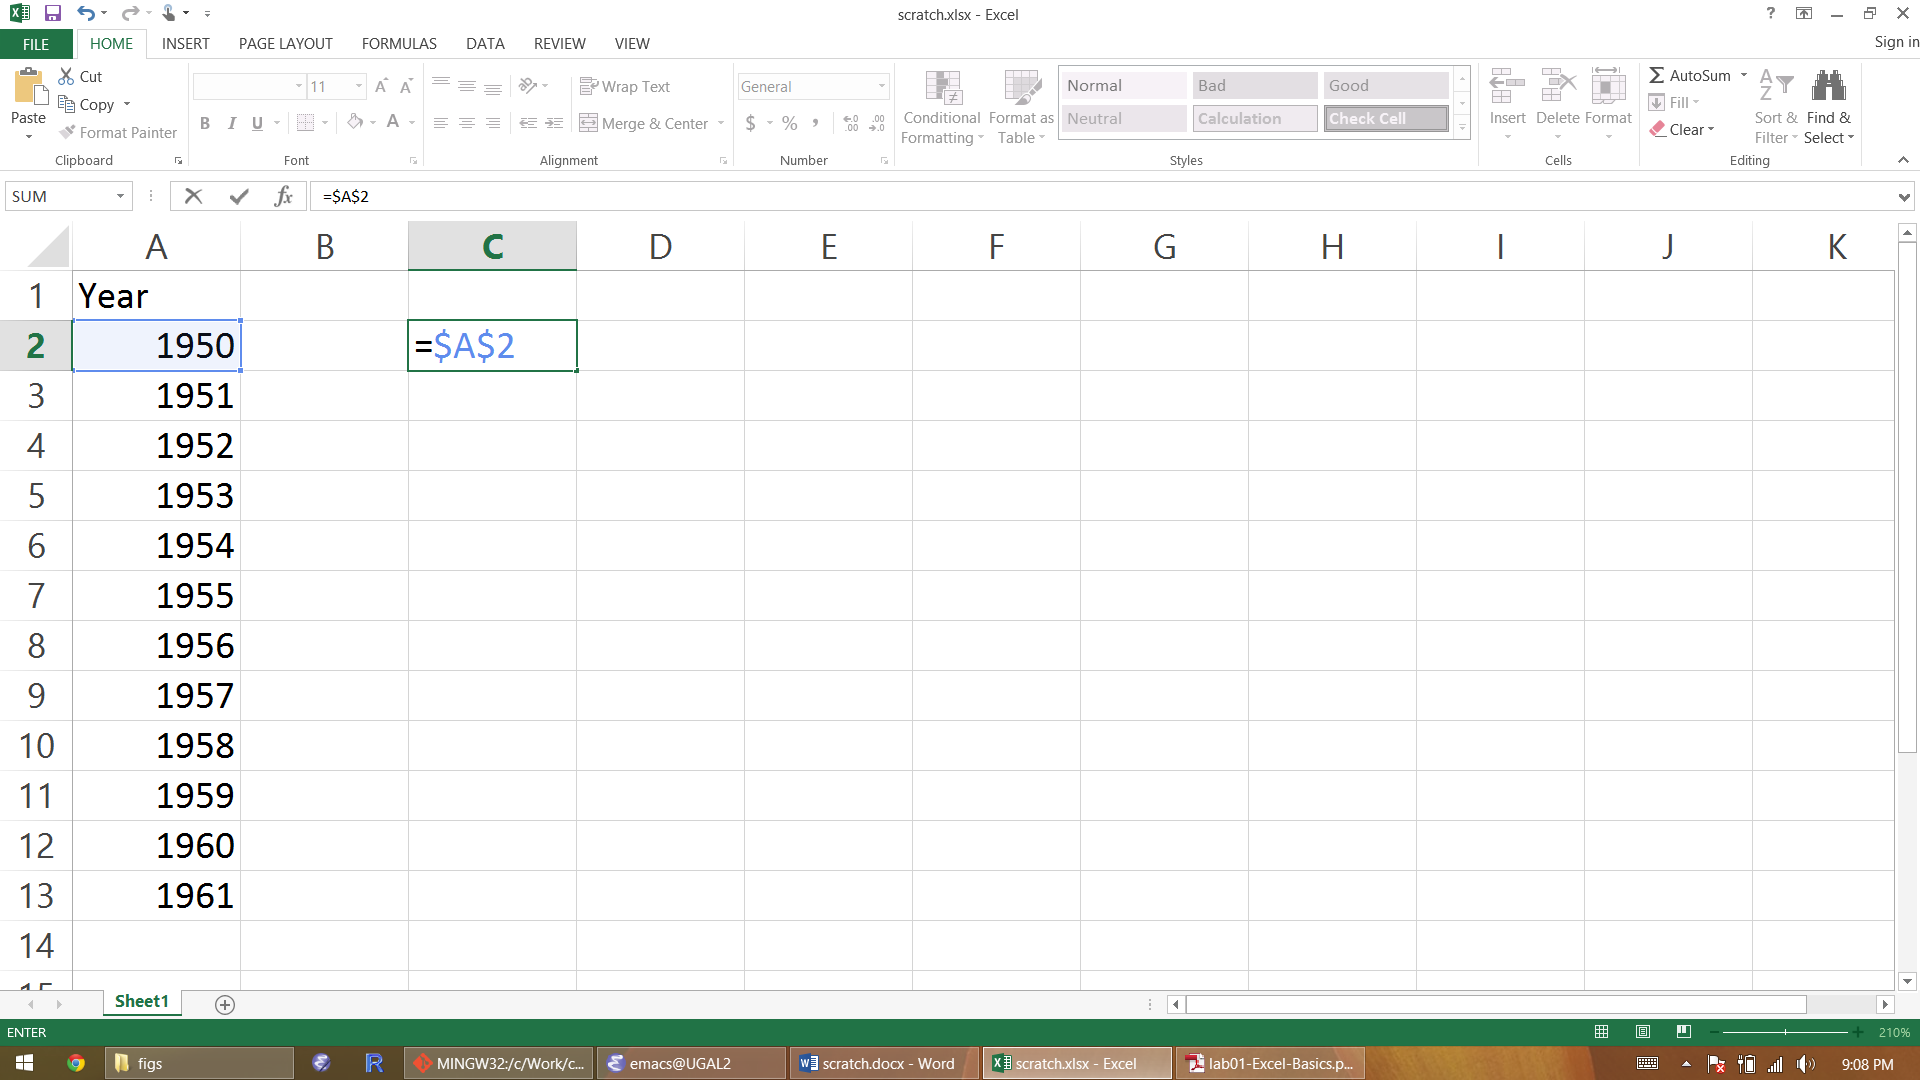
\includegraphics[width=\textwidth]{figs/absolute-ref}}}
  \only<2 | handout:0>{\fbox{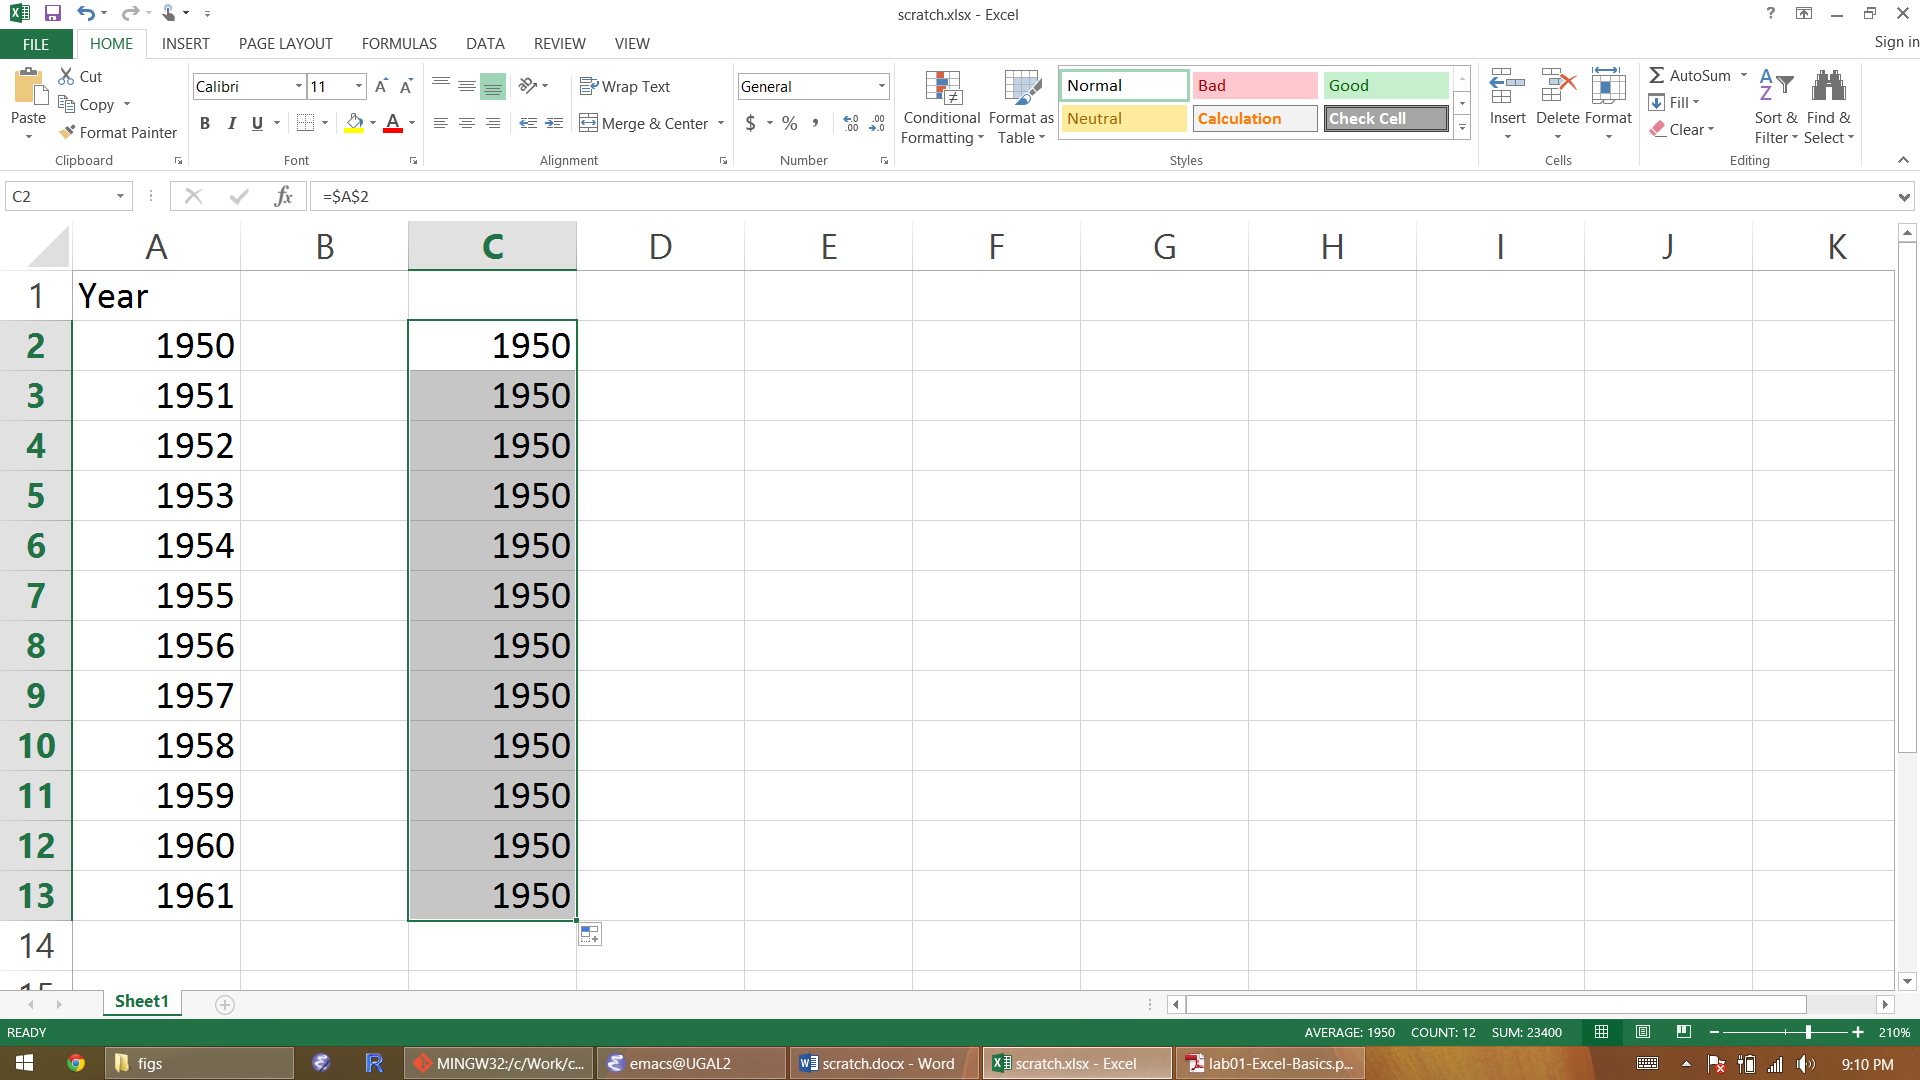
\includegraphics[width=\textwidth]{figs/absolute-ref2}}}
  \begin{center}
    Dollar sign ``locks'' value so that auto-fill won't change it
  \end{center}
\end{frame}


\begin{frame}
  \frametitle{Partial Cell References}
  \fbox{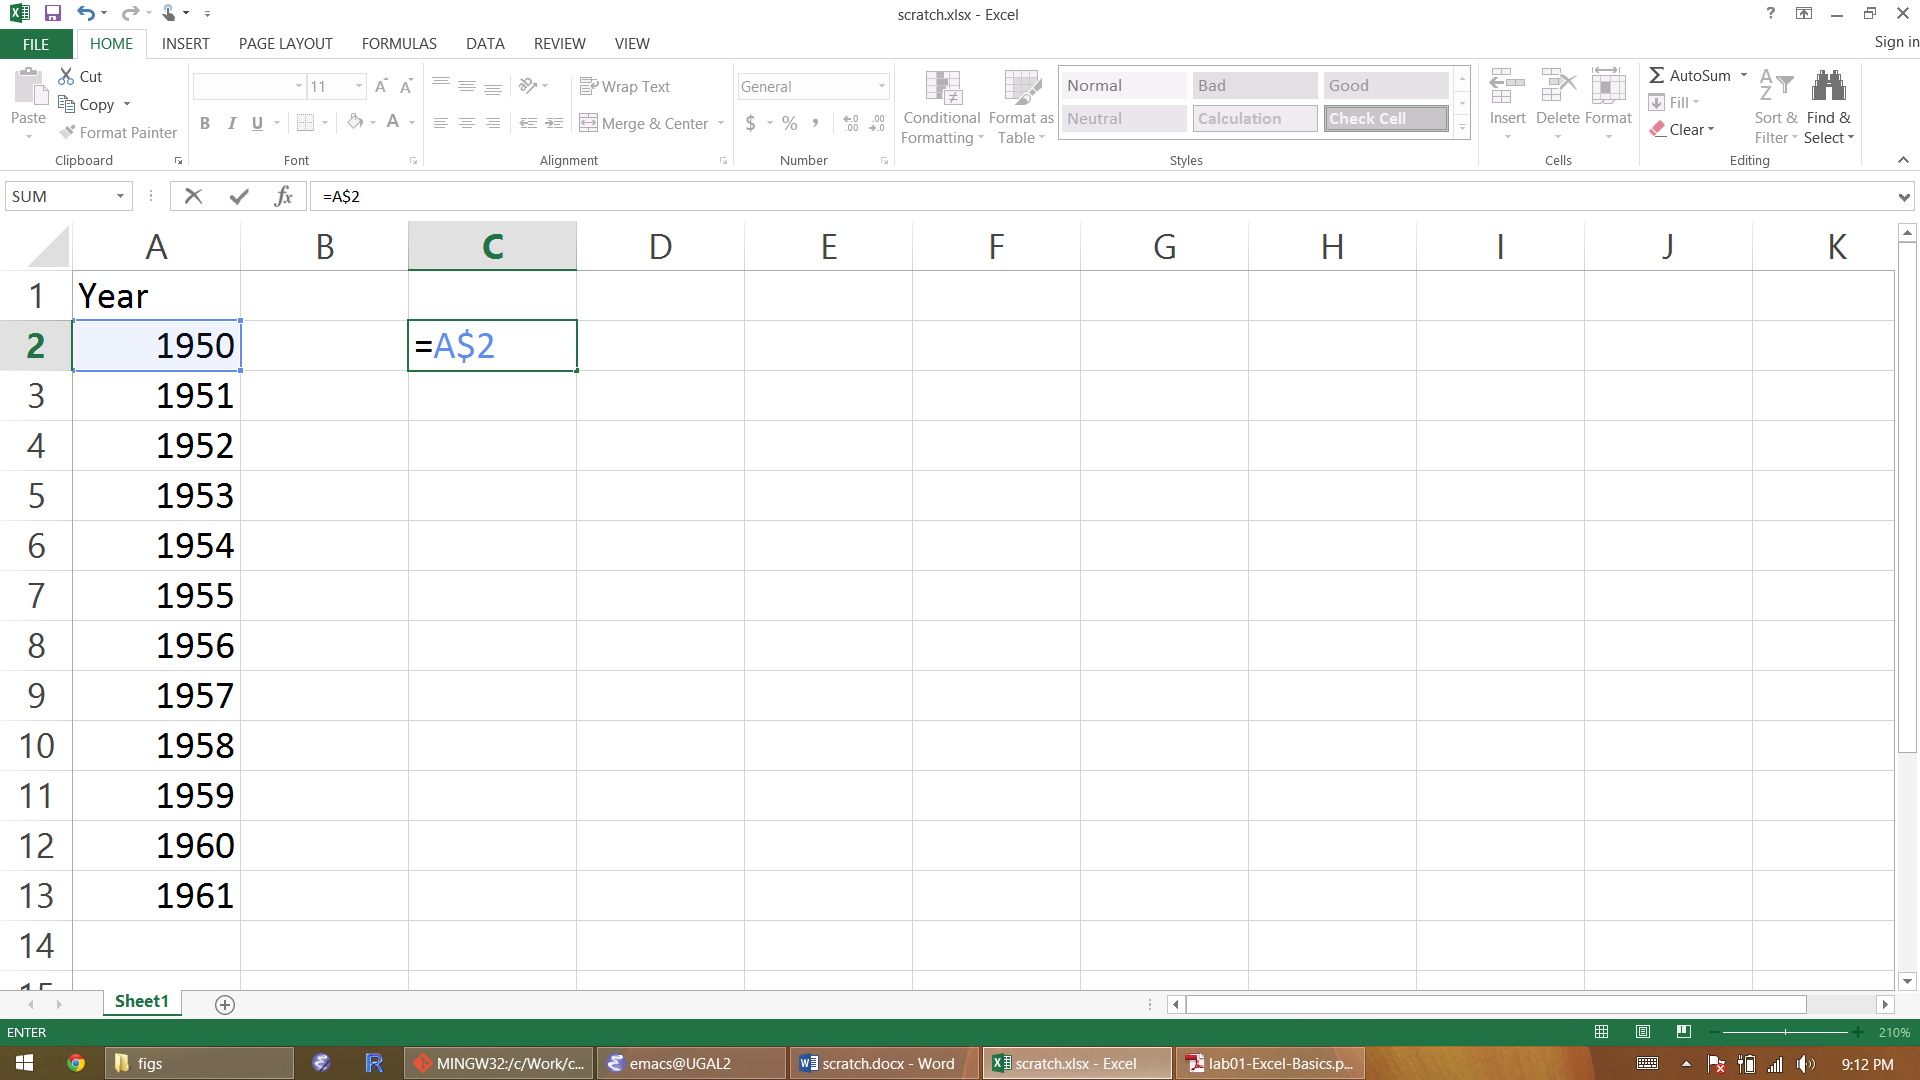
\includegraphics[width=\textwidth]{figs/partial-ref}}
\end{frame}


\section{Equations}



\begin{frame}
  \frametitle{Equations}
%  \begin{ce}
    \only<1>{\fbox{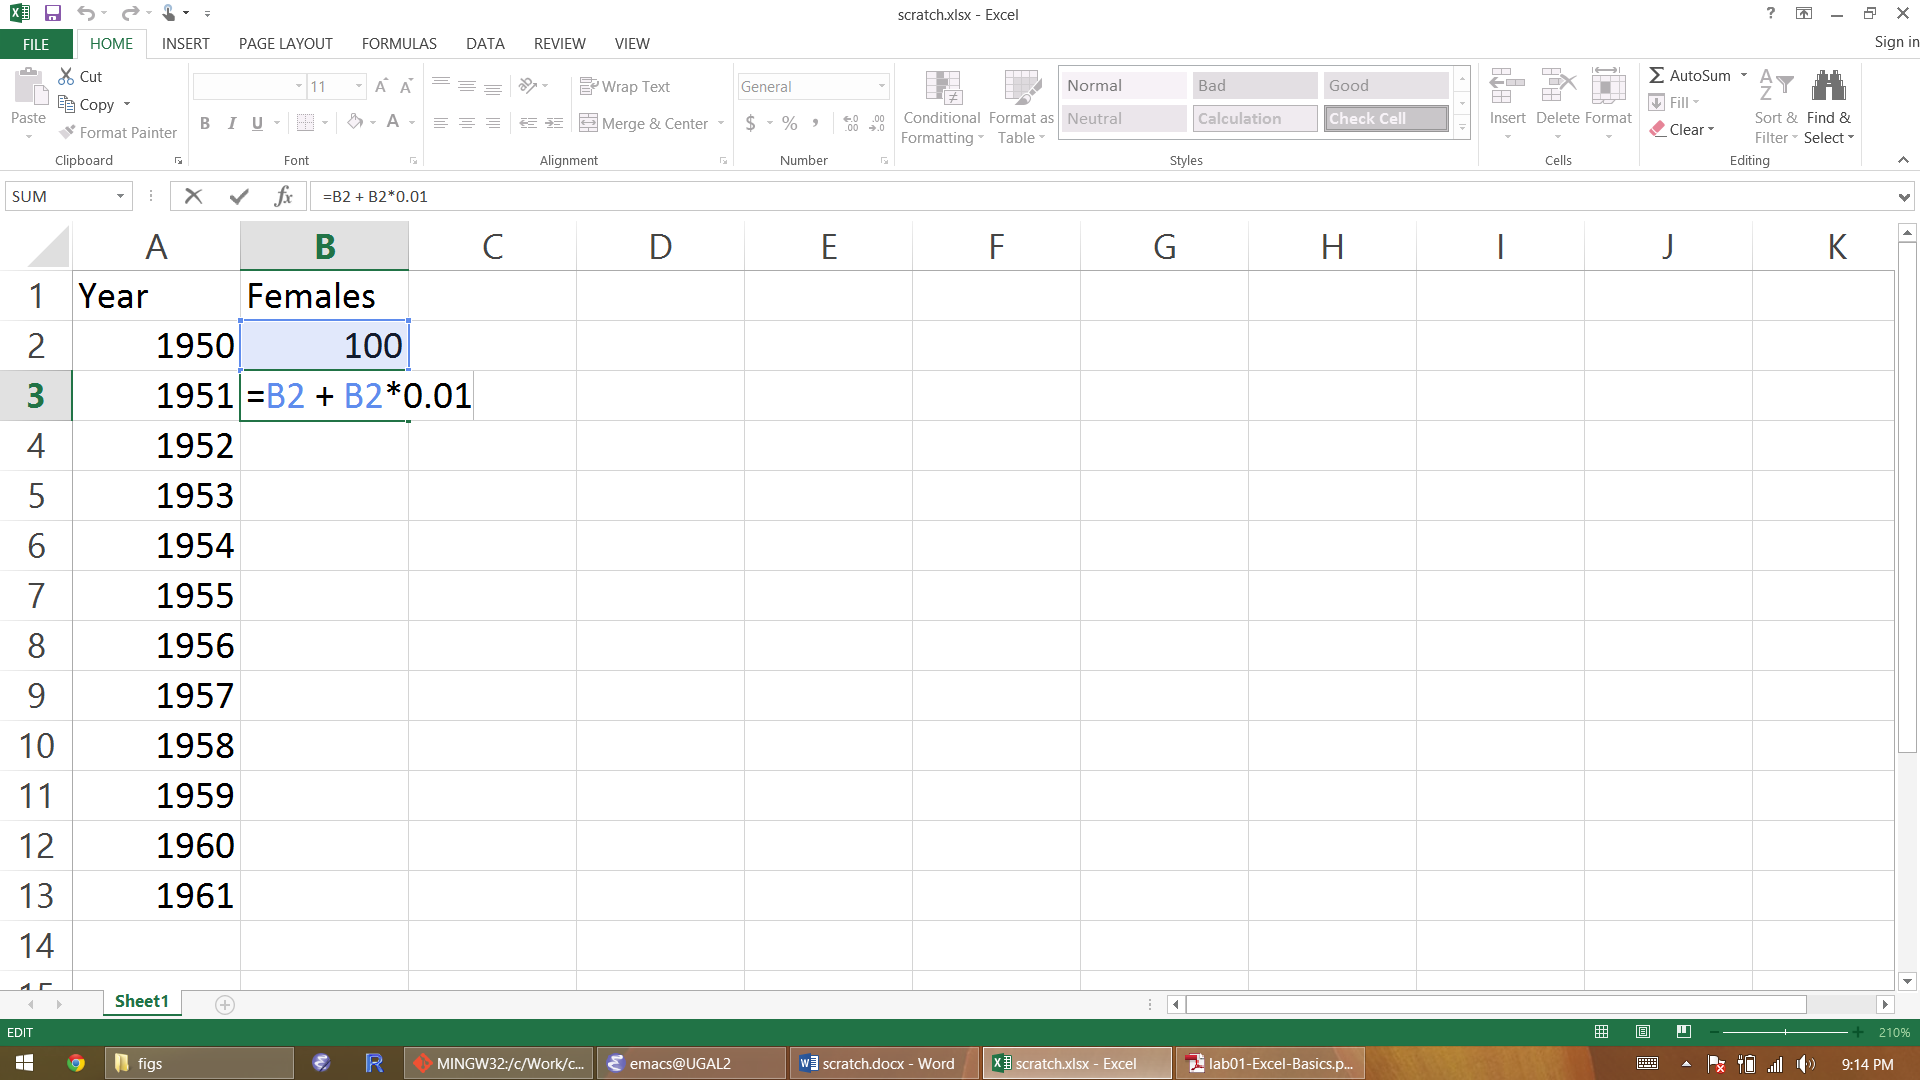
\includegraphics[width=\textwidth]{figs/equation}}}
    \only<2 | handout:0>{\fbox{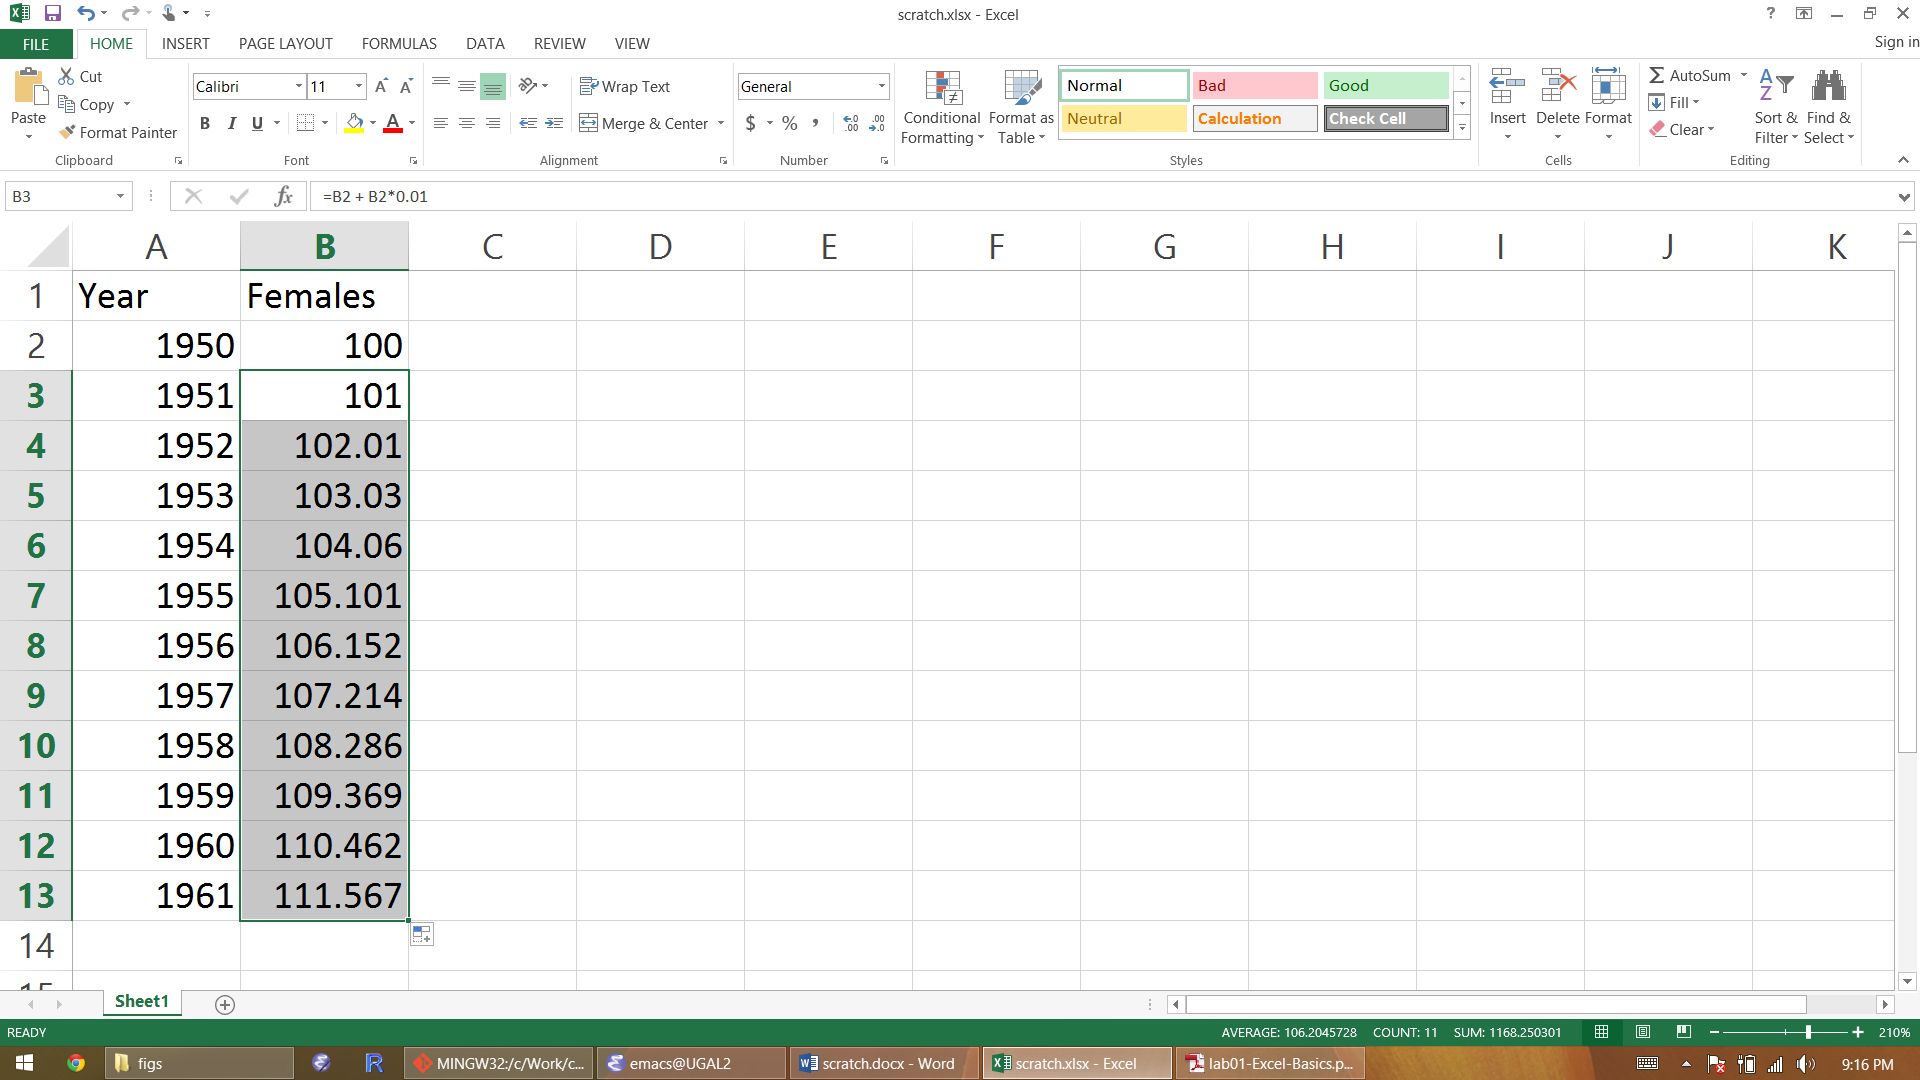
\includegraphics[width=\textwidth]{figs/equation2}}}
%  \end{overprint}
\end{frame}



\begin{frame}
  \frametitle{Equations}
    \only<1>{\fbox{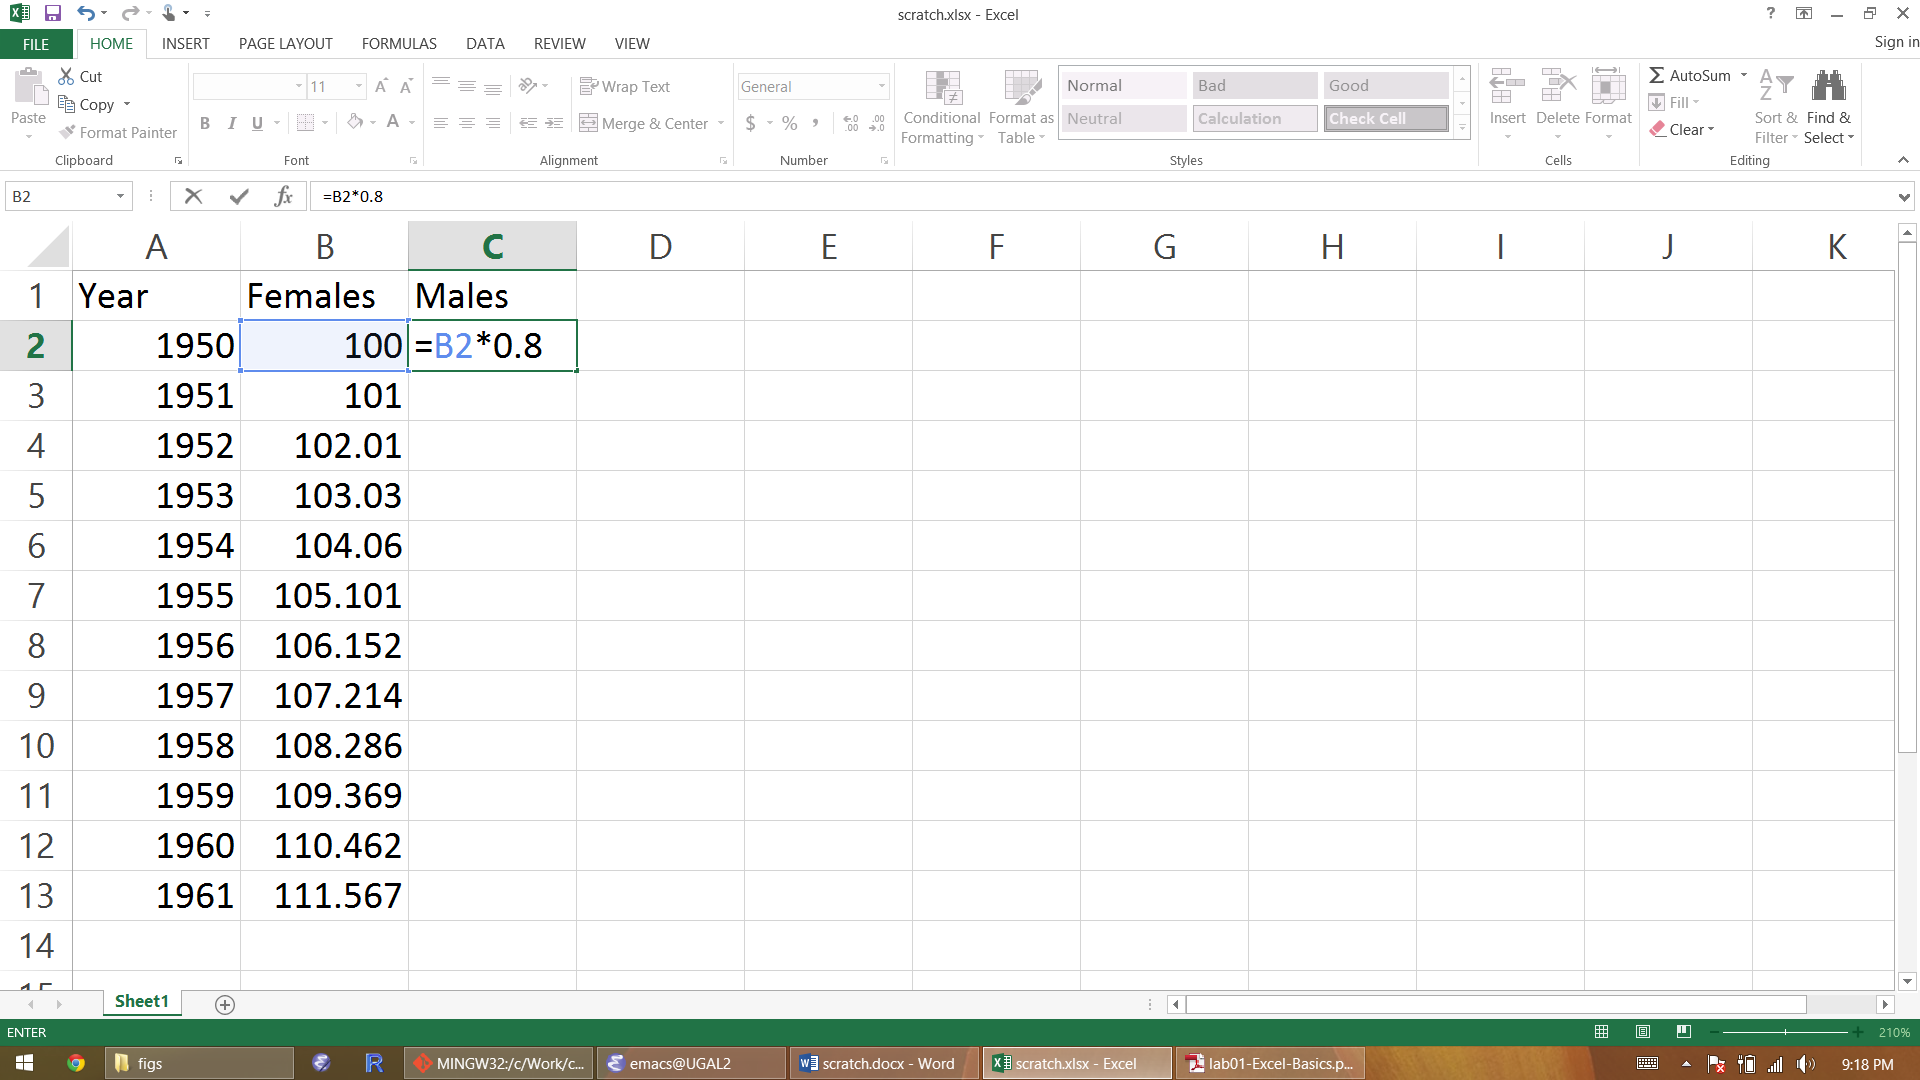
\includegraphics[width=\textwidth]{figs/equation3}}}
    \only<2 | handout:0>{\fbox{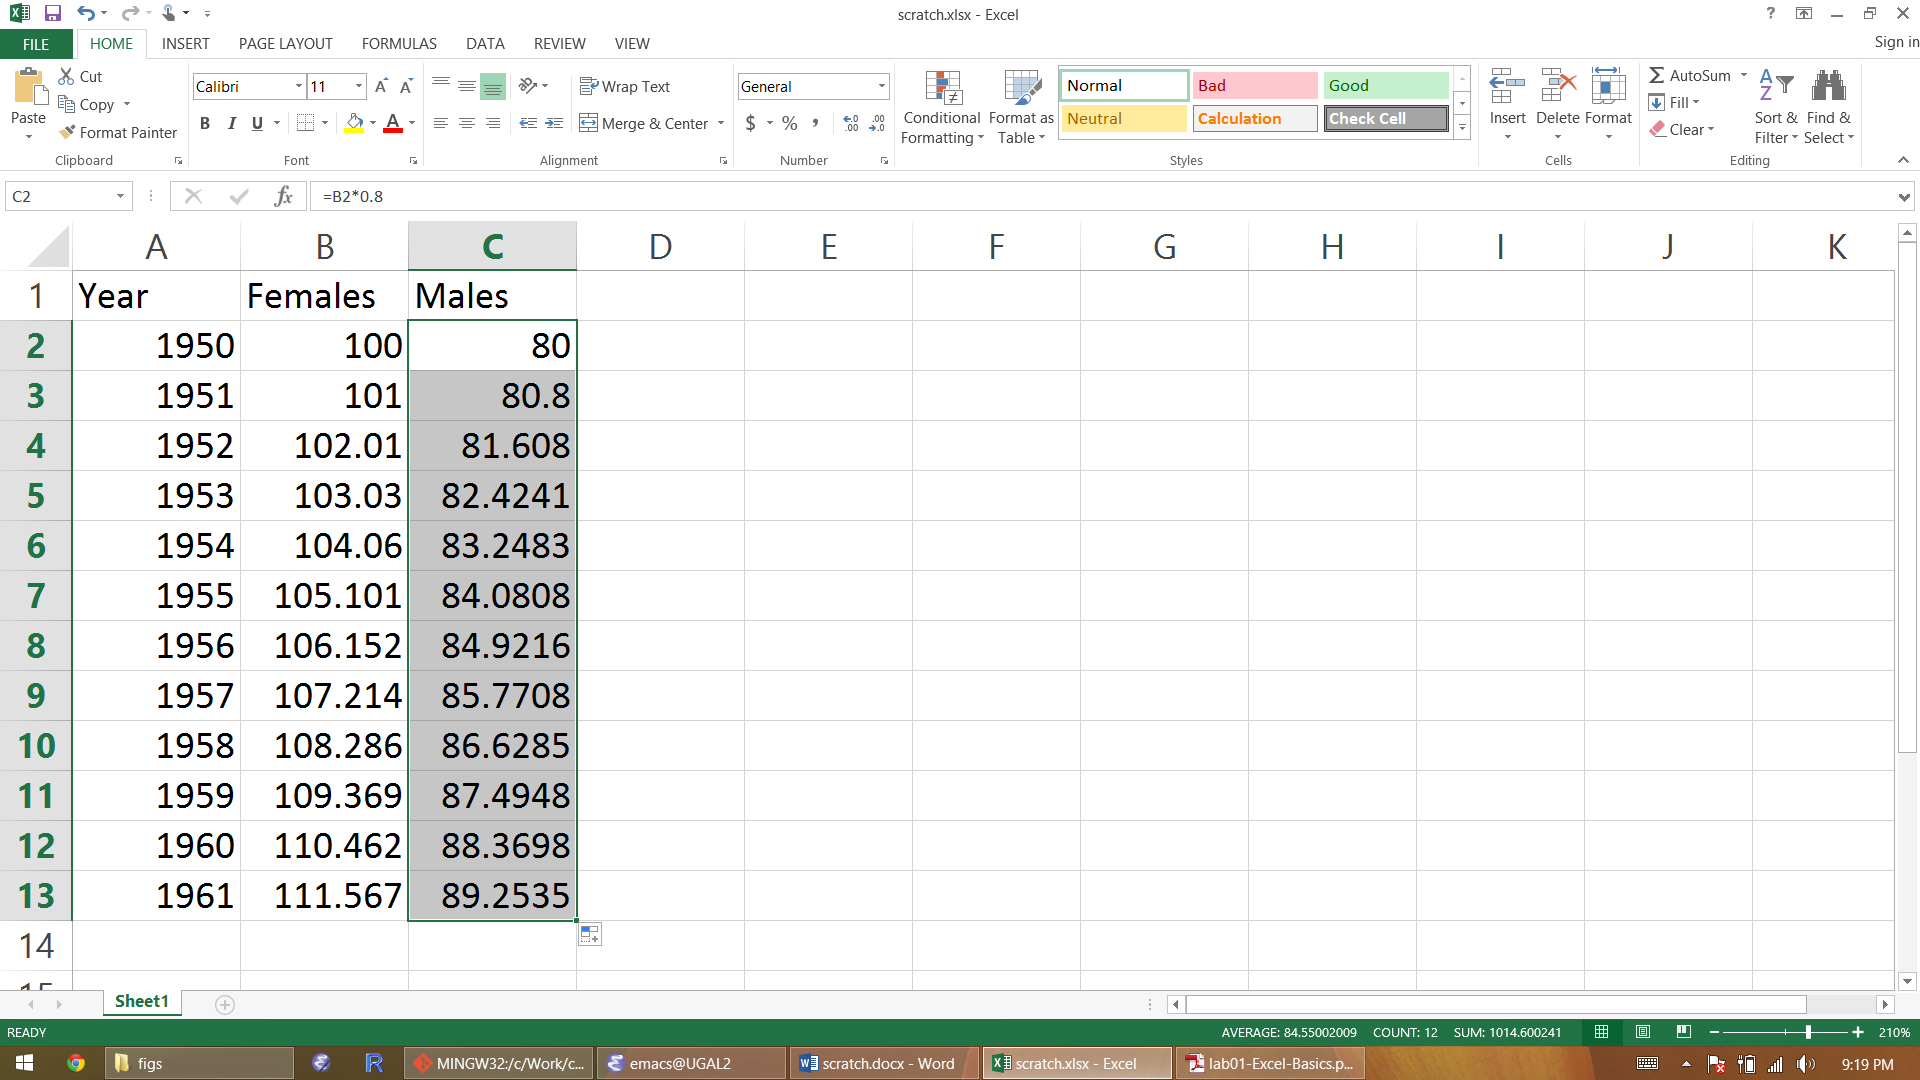
\includegraphics[width=\textwidth]{figs/equation4}}}
\end{frame}



\begin{frame}
  \frametitle{Formulas}
  \fbox{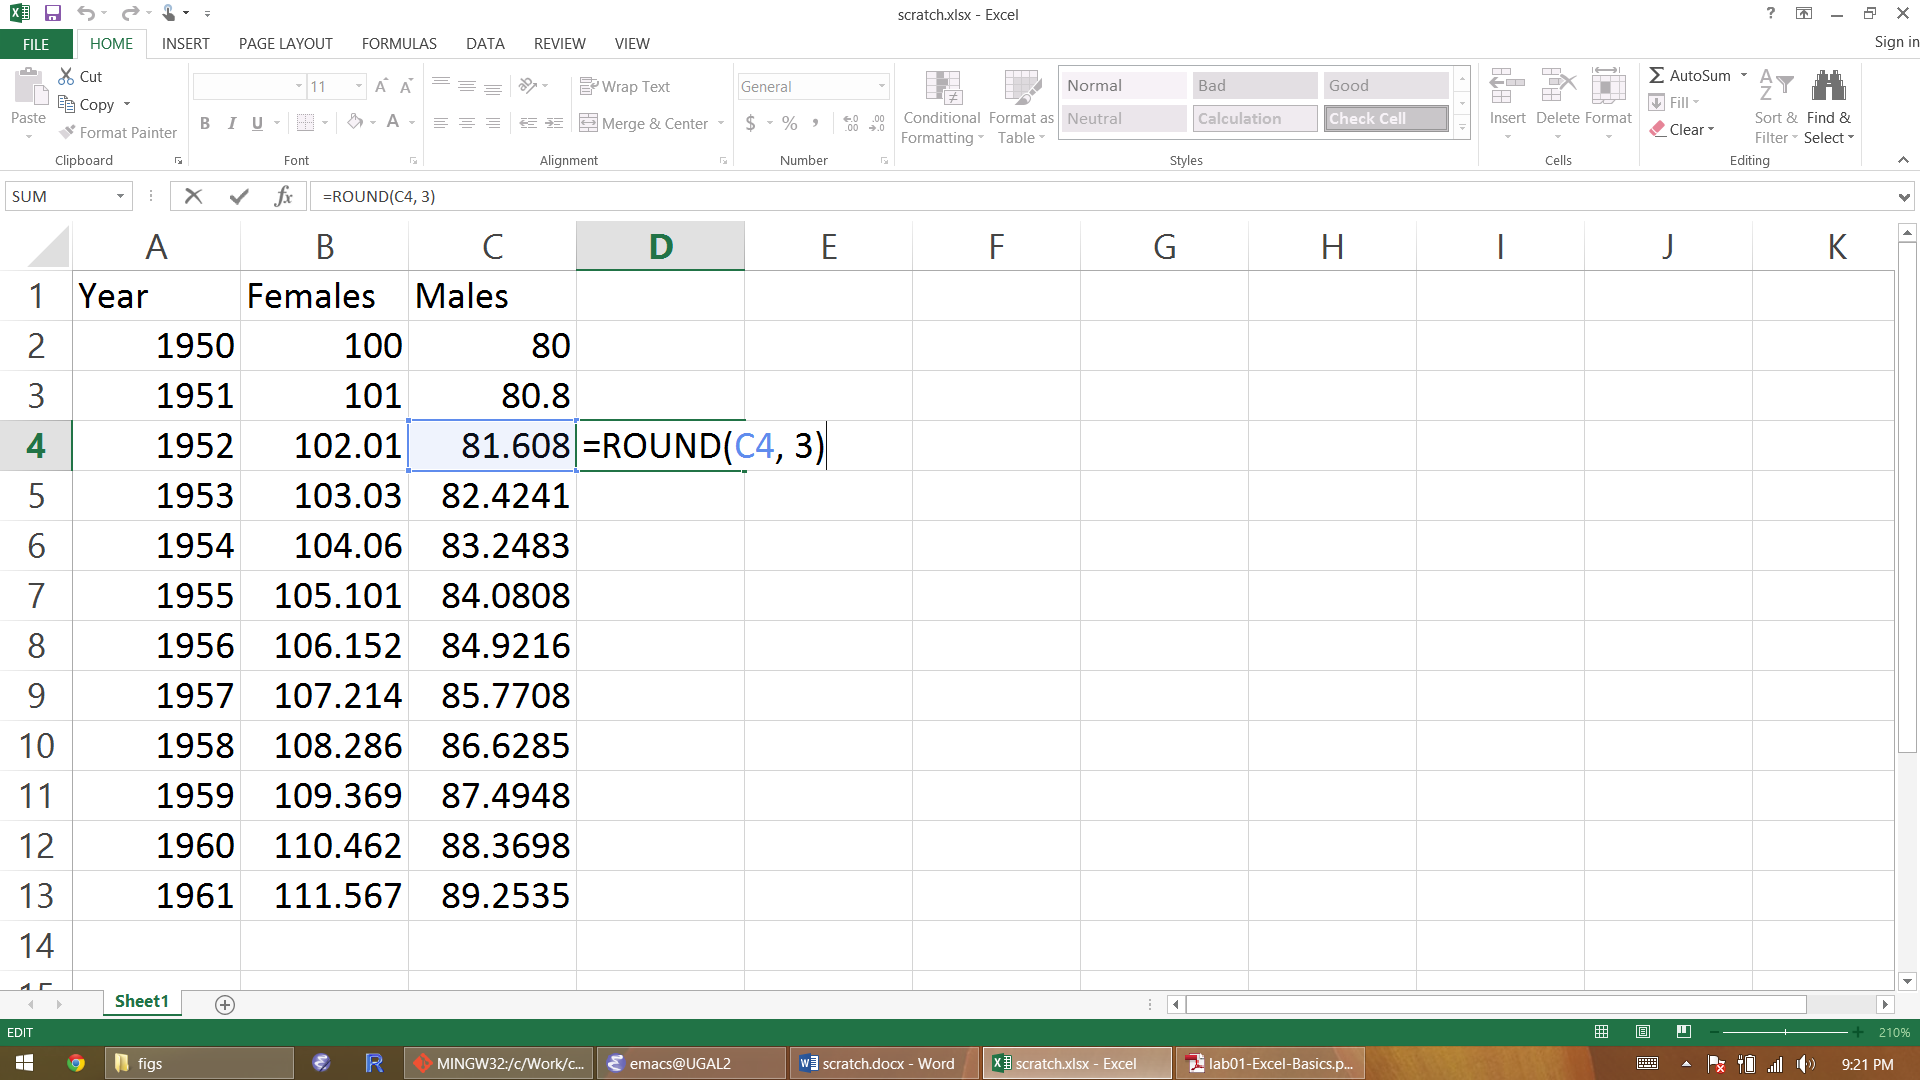
\includegraphics[width=\textwidth]{figs/formula}}
\end{frame}


\section{Graphics}



\begin{frame}
  \frametitle{Graphics}
%  \begin{overprint}
    \fbox{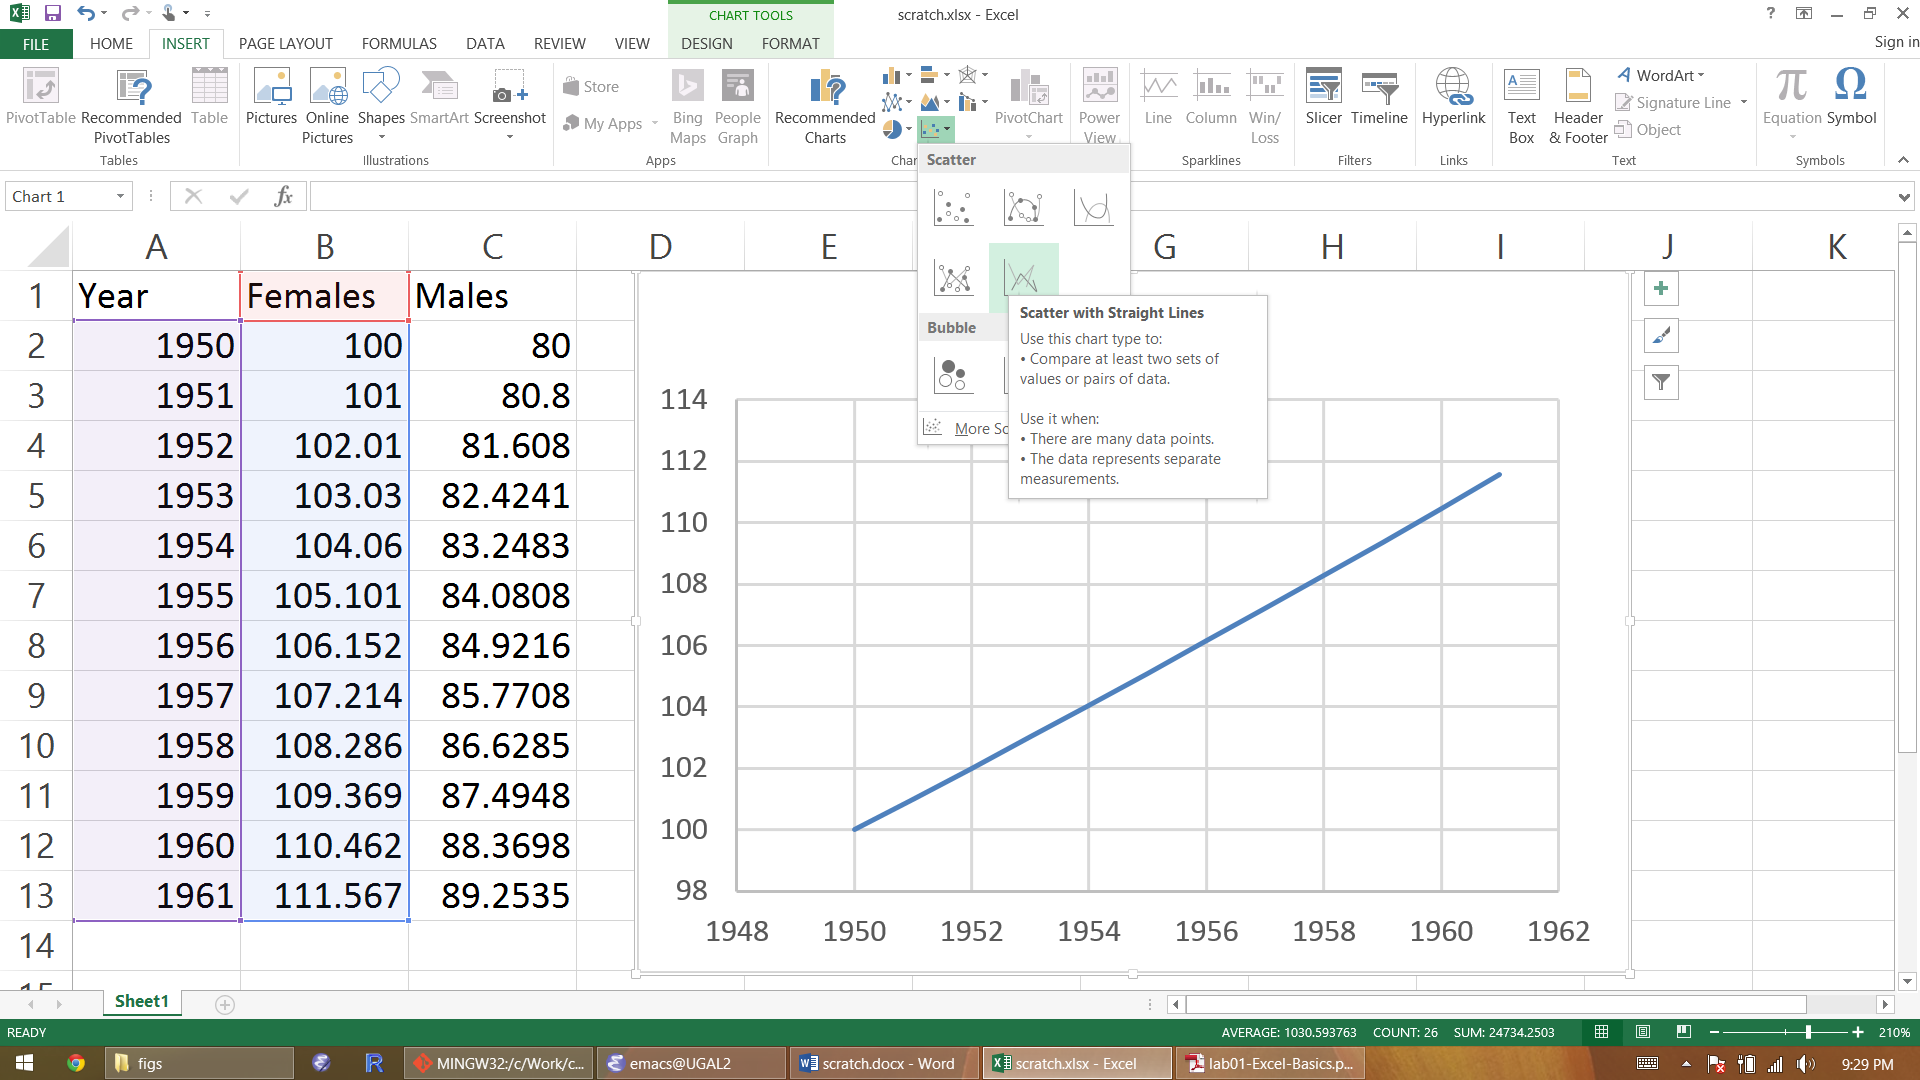
\includegraphics[width=\textwidth]{figs/scatterlines}}
%    \only<2 | handout:0>{\fbox{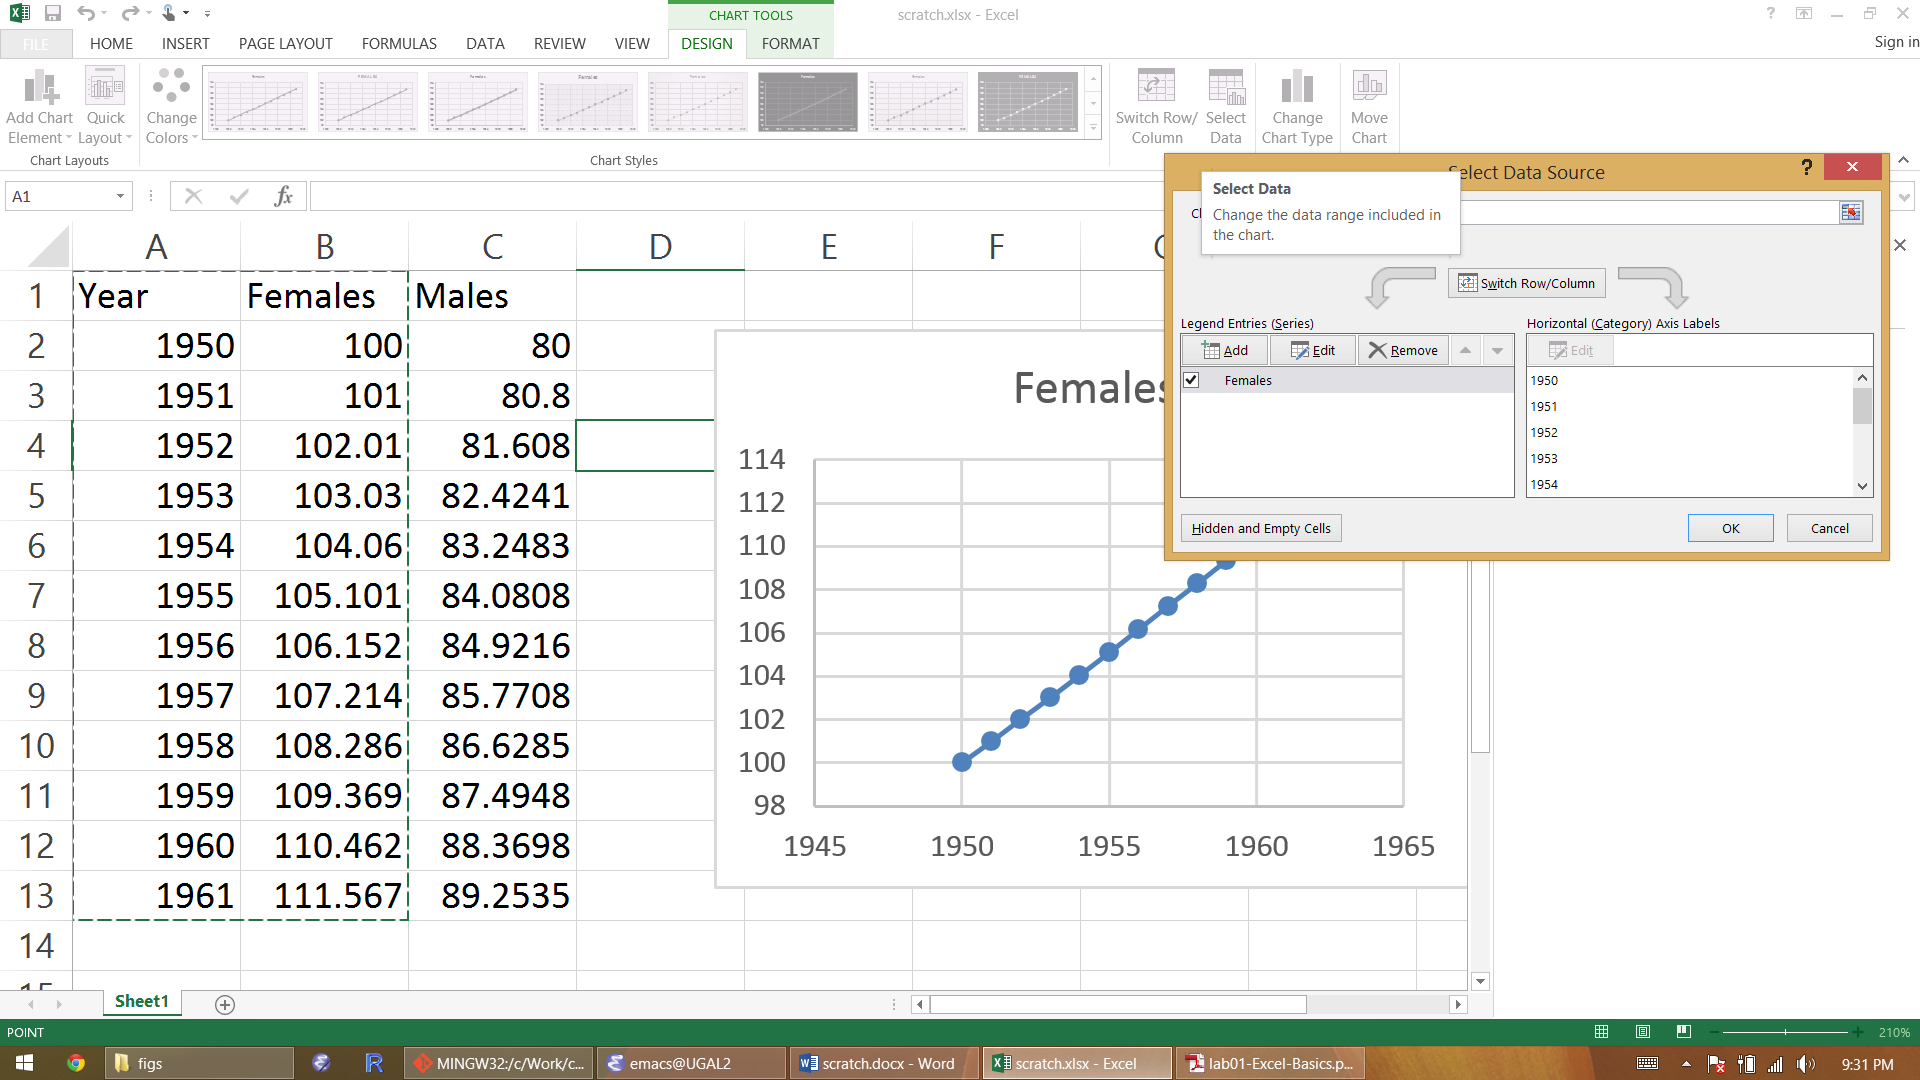
\includegraphics[width=\textwidth]{figs/scatterlines2}}}
%  \end{overprint}
\end{frame}


\begin{frame}
  \frametitle{Graphics}
  \only<1>{\fbox{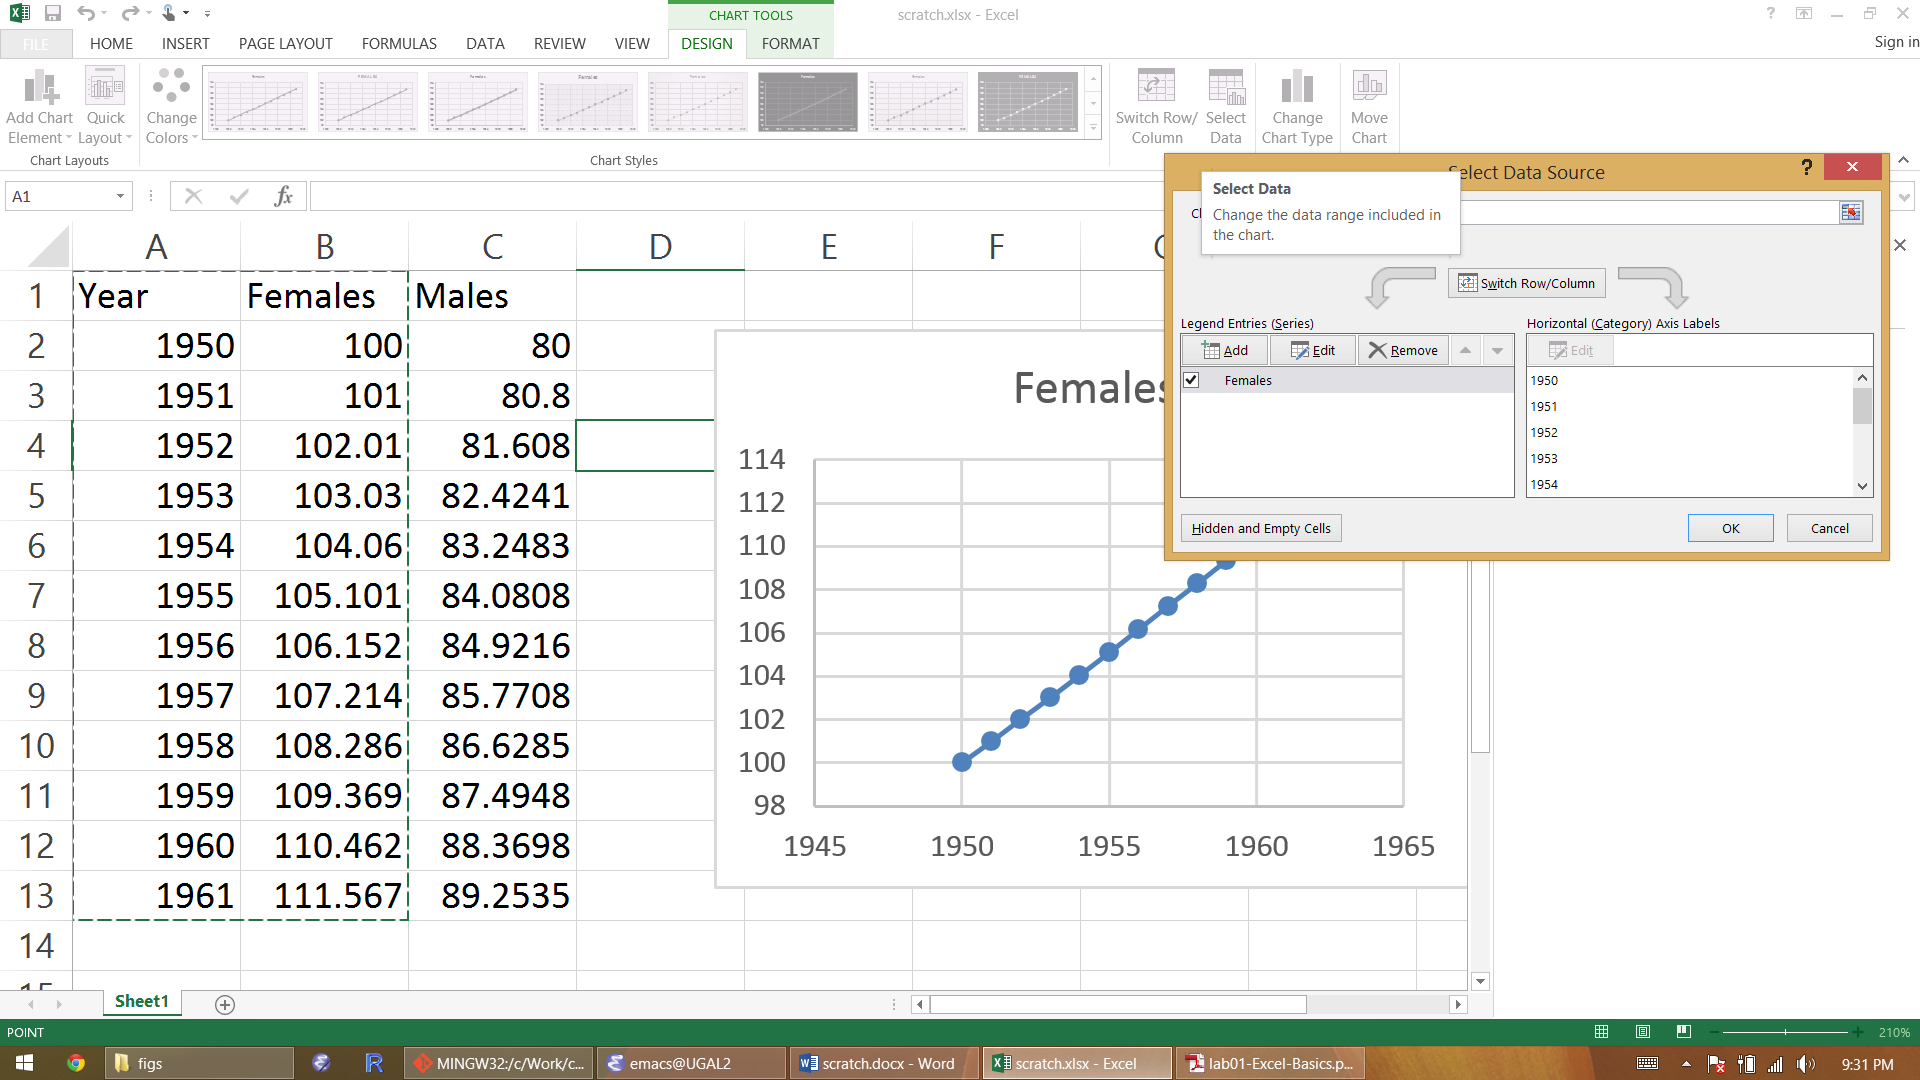
\includegraphics[width=\textwidth]{figs/scatterlines2}}}
  \only<2>{\fbox{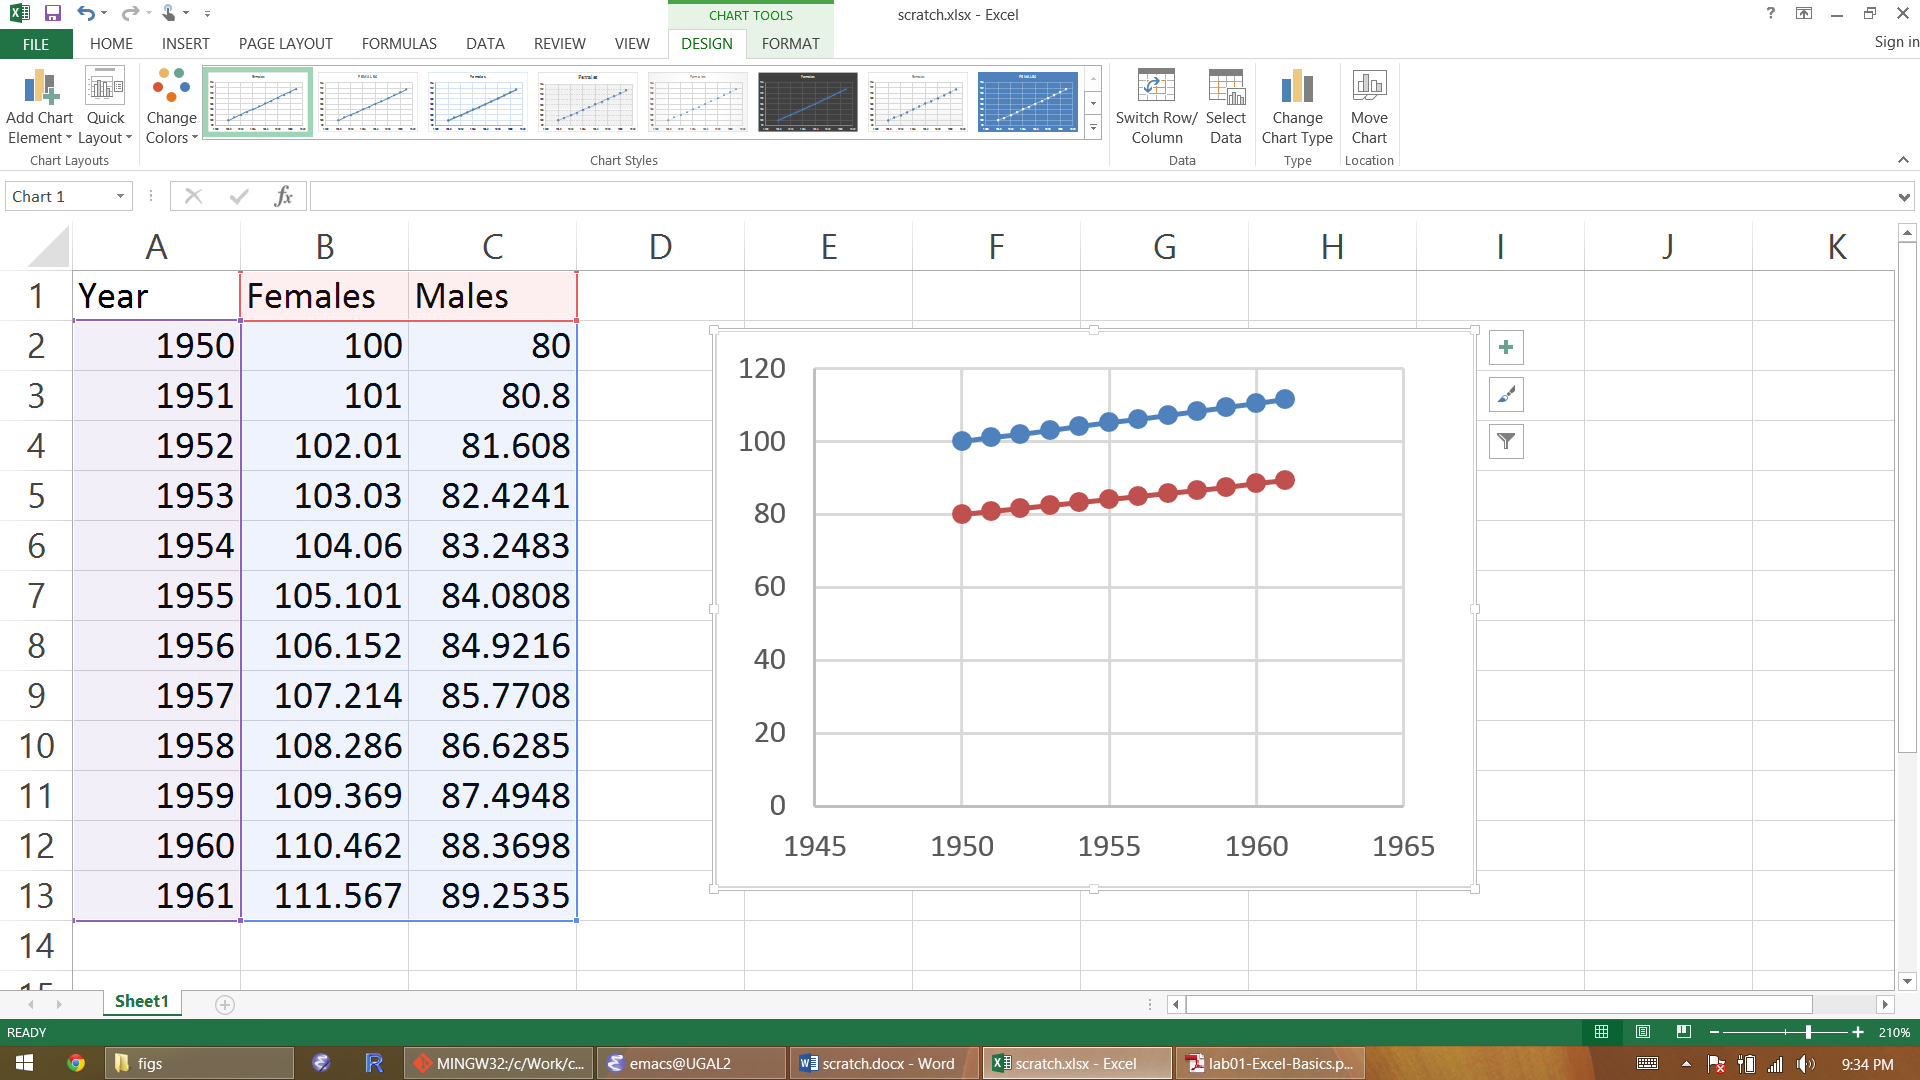
\includegraphics[width=\textwidth]{figs/scatterlines3}}}
  \begin{center}
    Add a line for males
  \end{center}
\end{frame}


% \begin{frame}
%   \frametitle{Add Headings}
%   \only<1>{\fbox{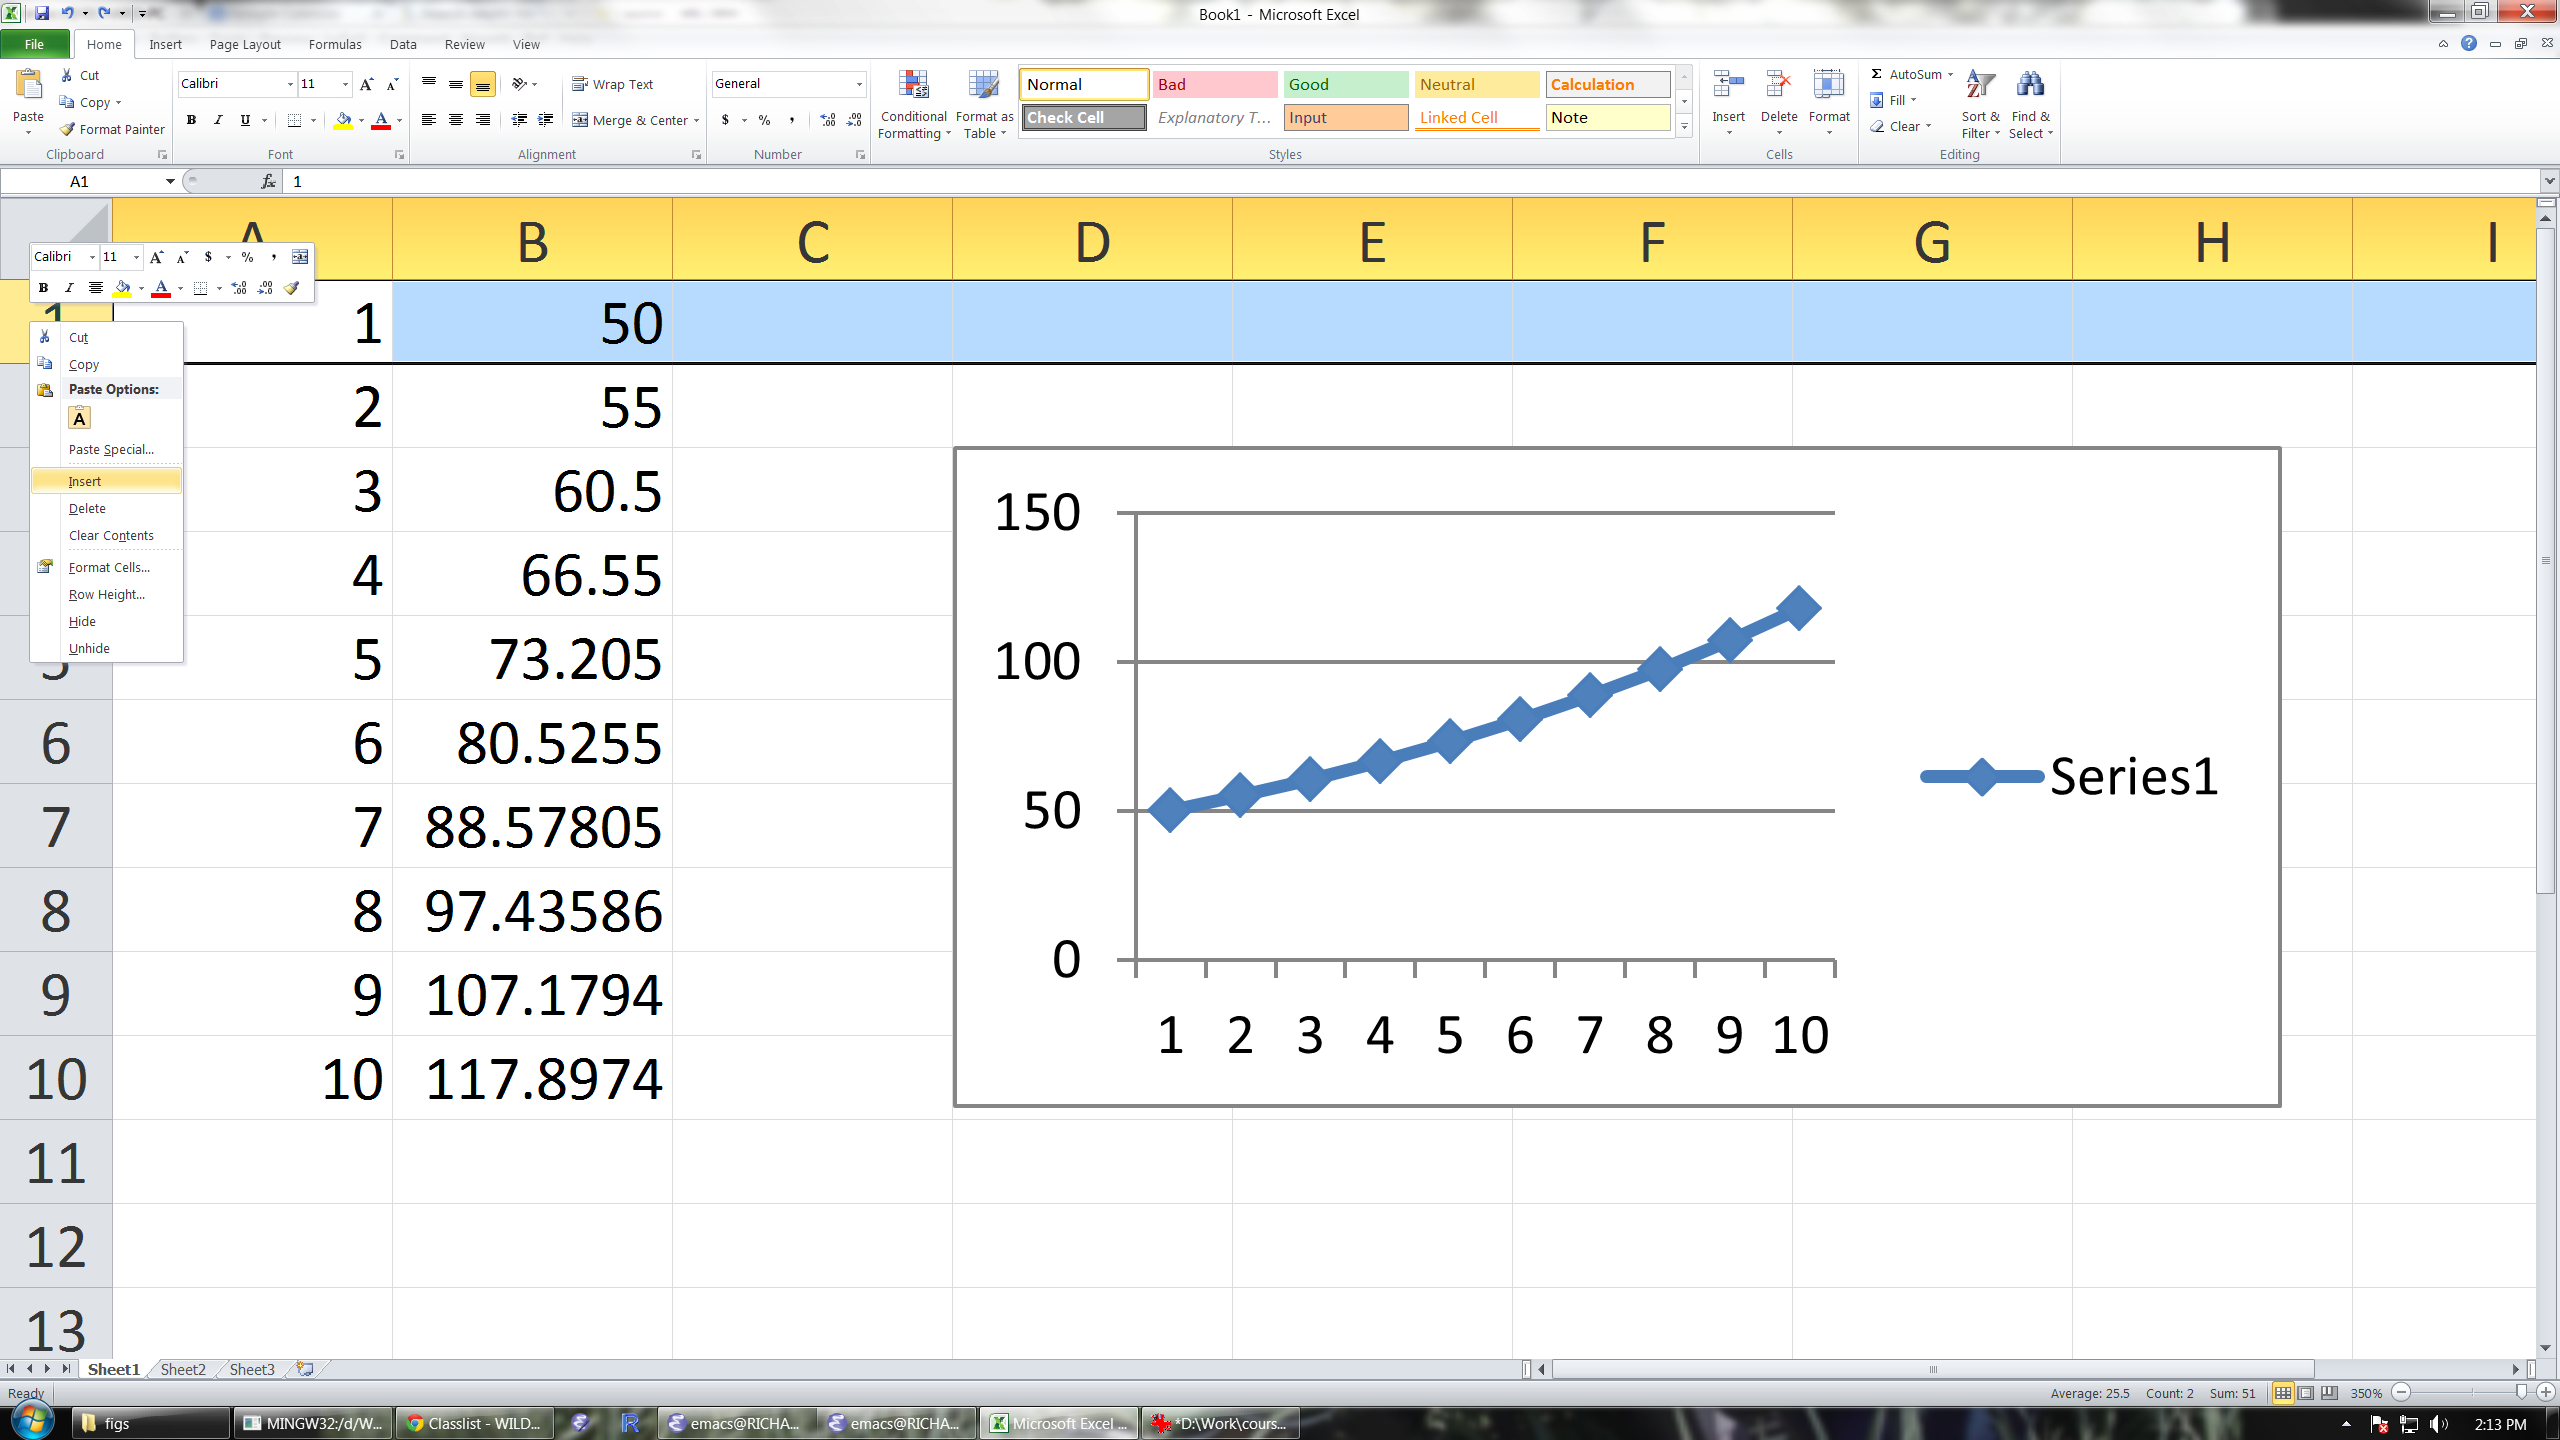
\includegraphics[width=\textwidth]{figs/headings}}}
%   \only<2>{\fbox{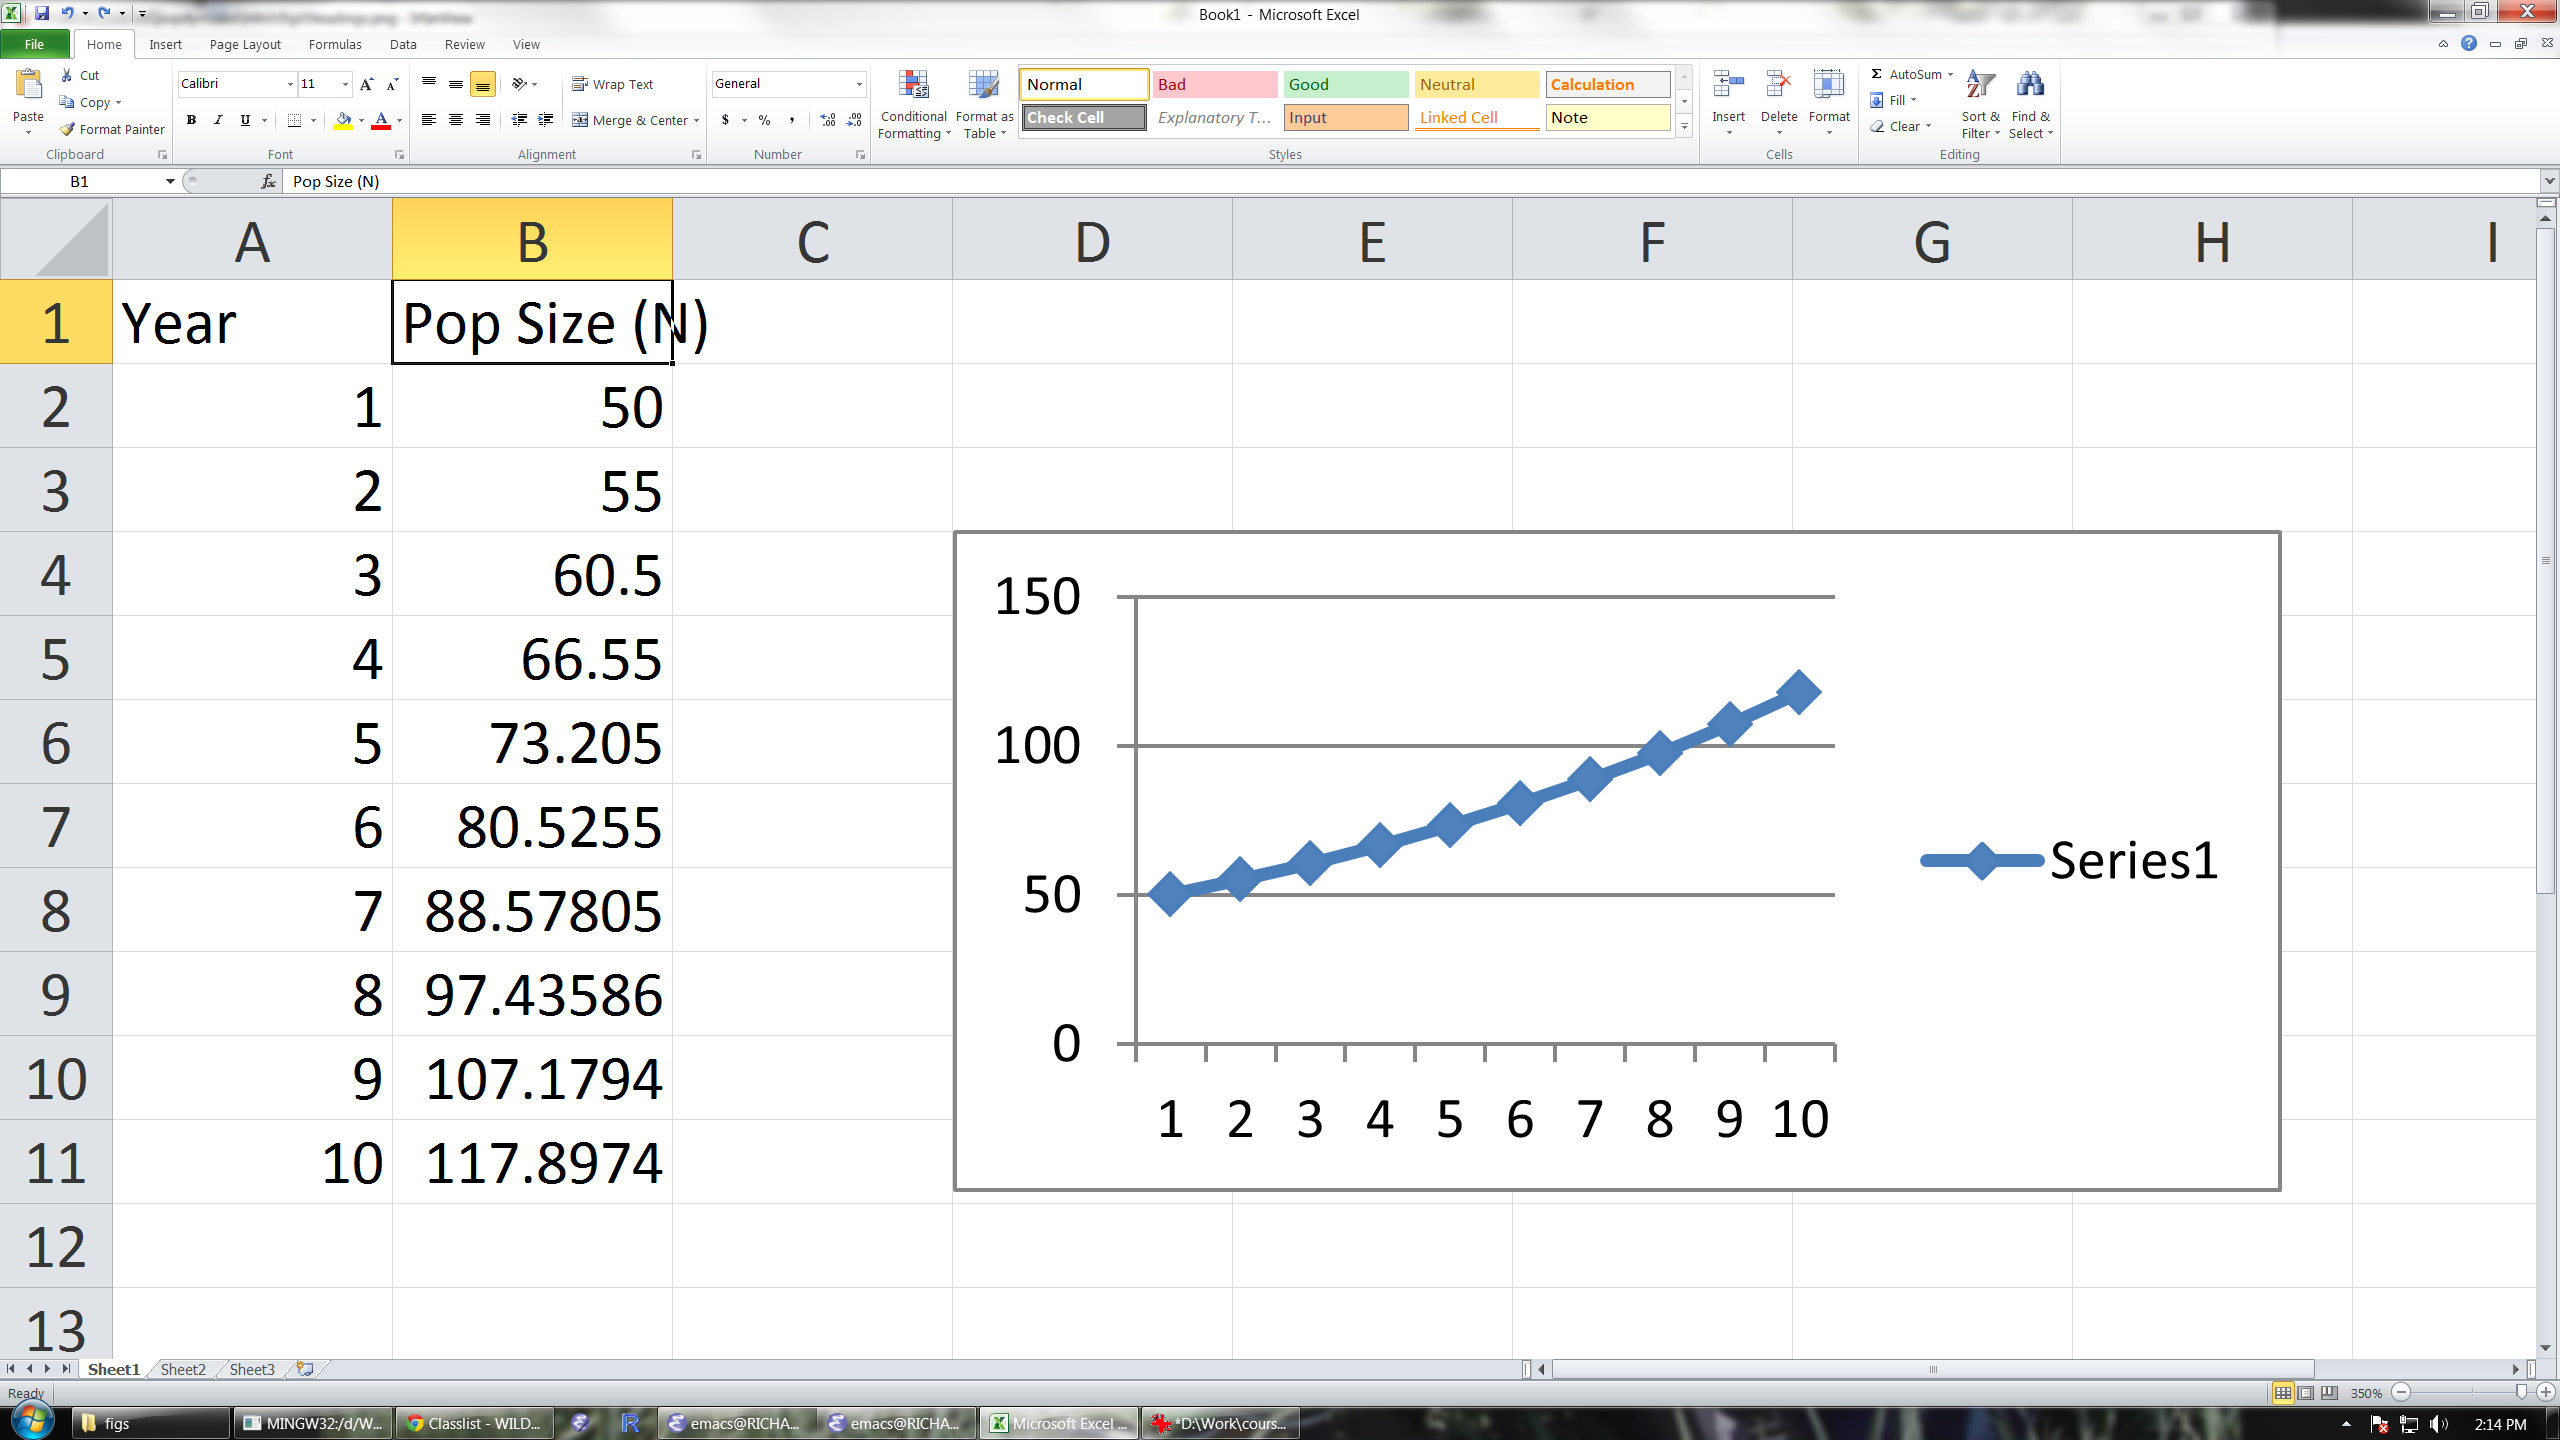
\includegraphics[width=\textwidth]{figs/headings2}}}
% \end{frame}



\begin{frame}
  \frametitle{Customize}
%  \begin{overprint}
    \only<1>{\fbox{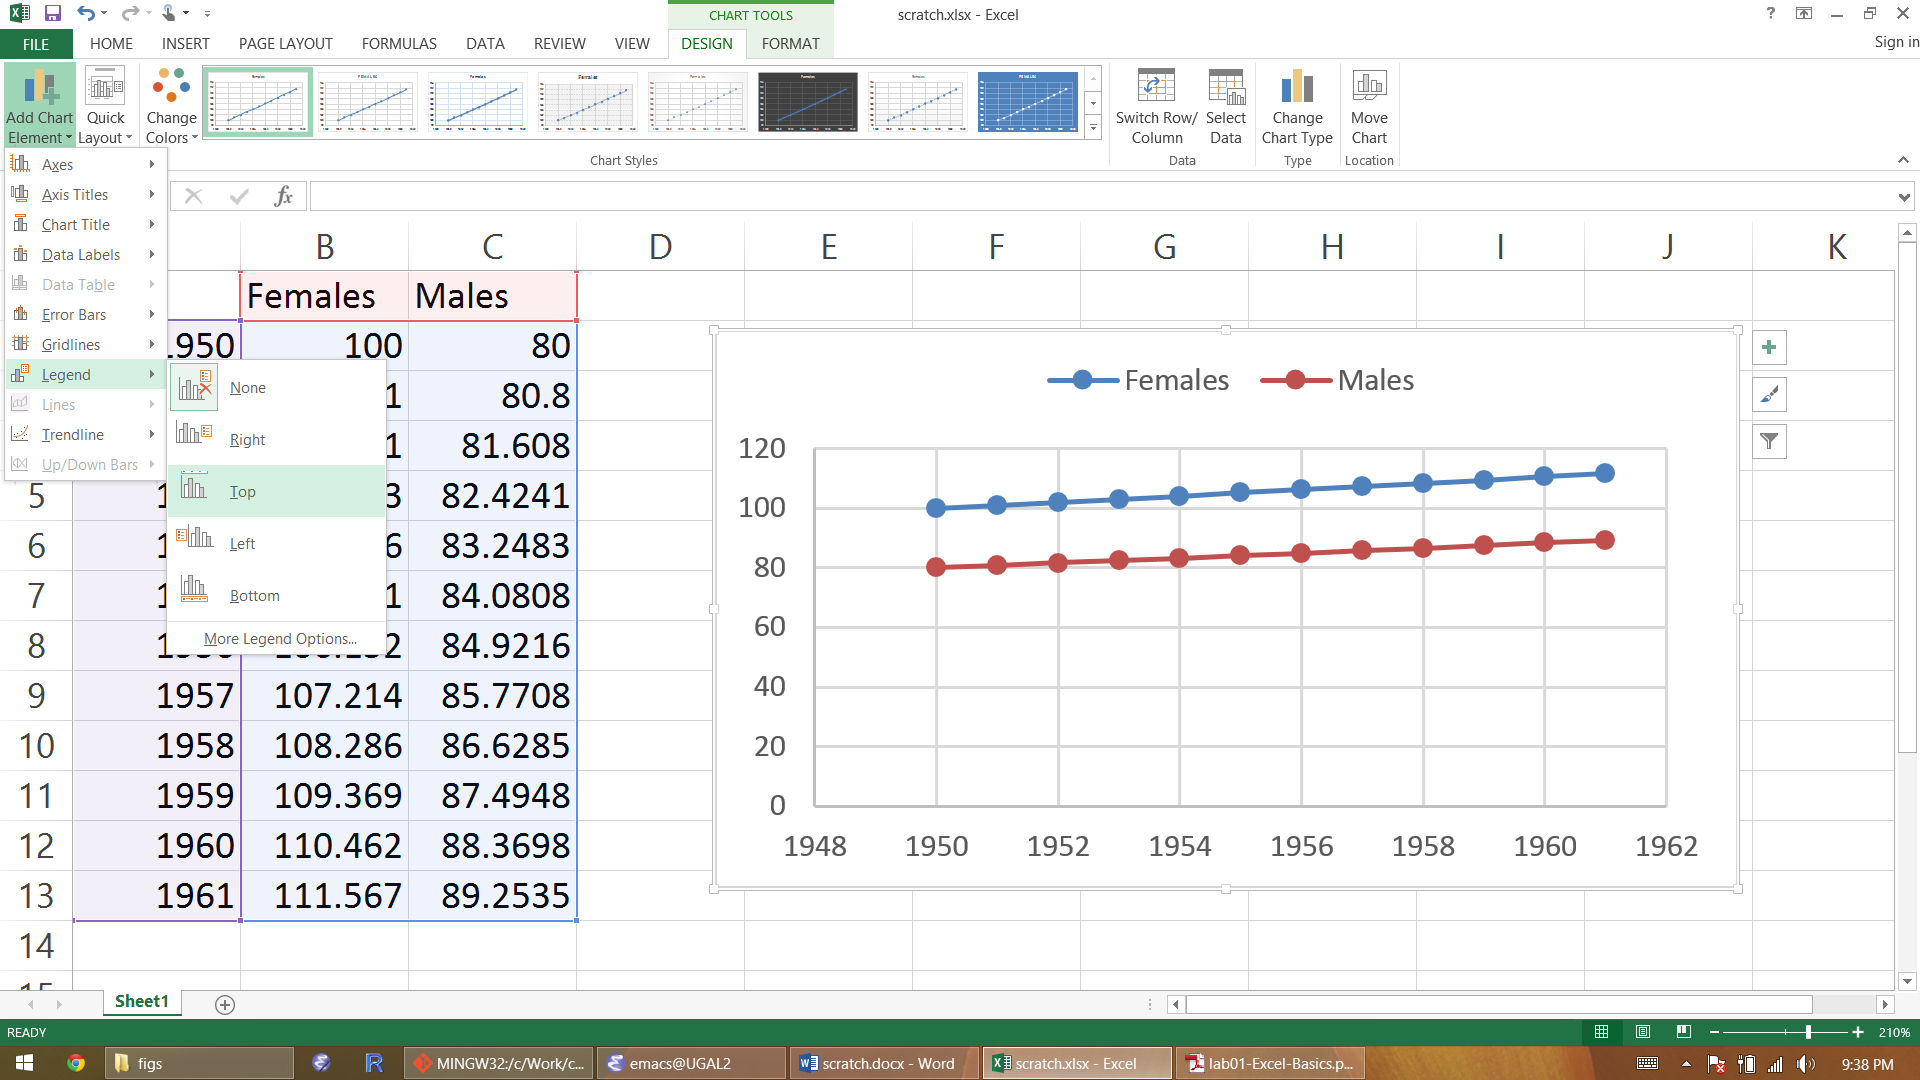
\includegraphics[width=\textwidth]{figs/customize}}}
%    \only<2 | handout:0>{\fbox{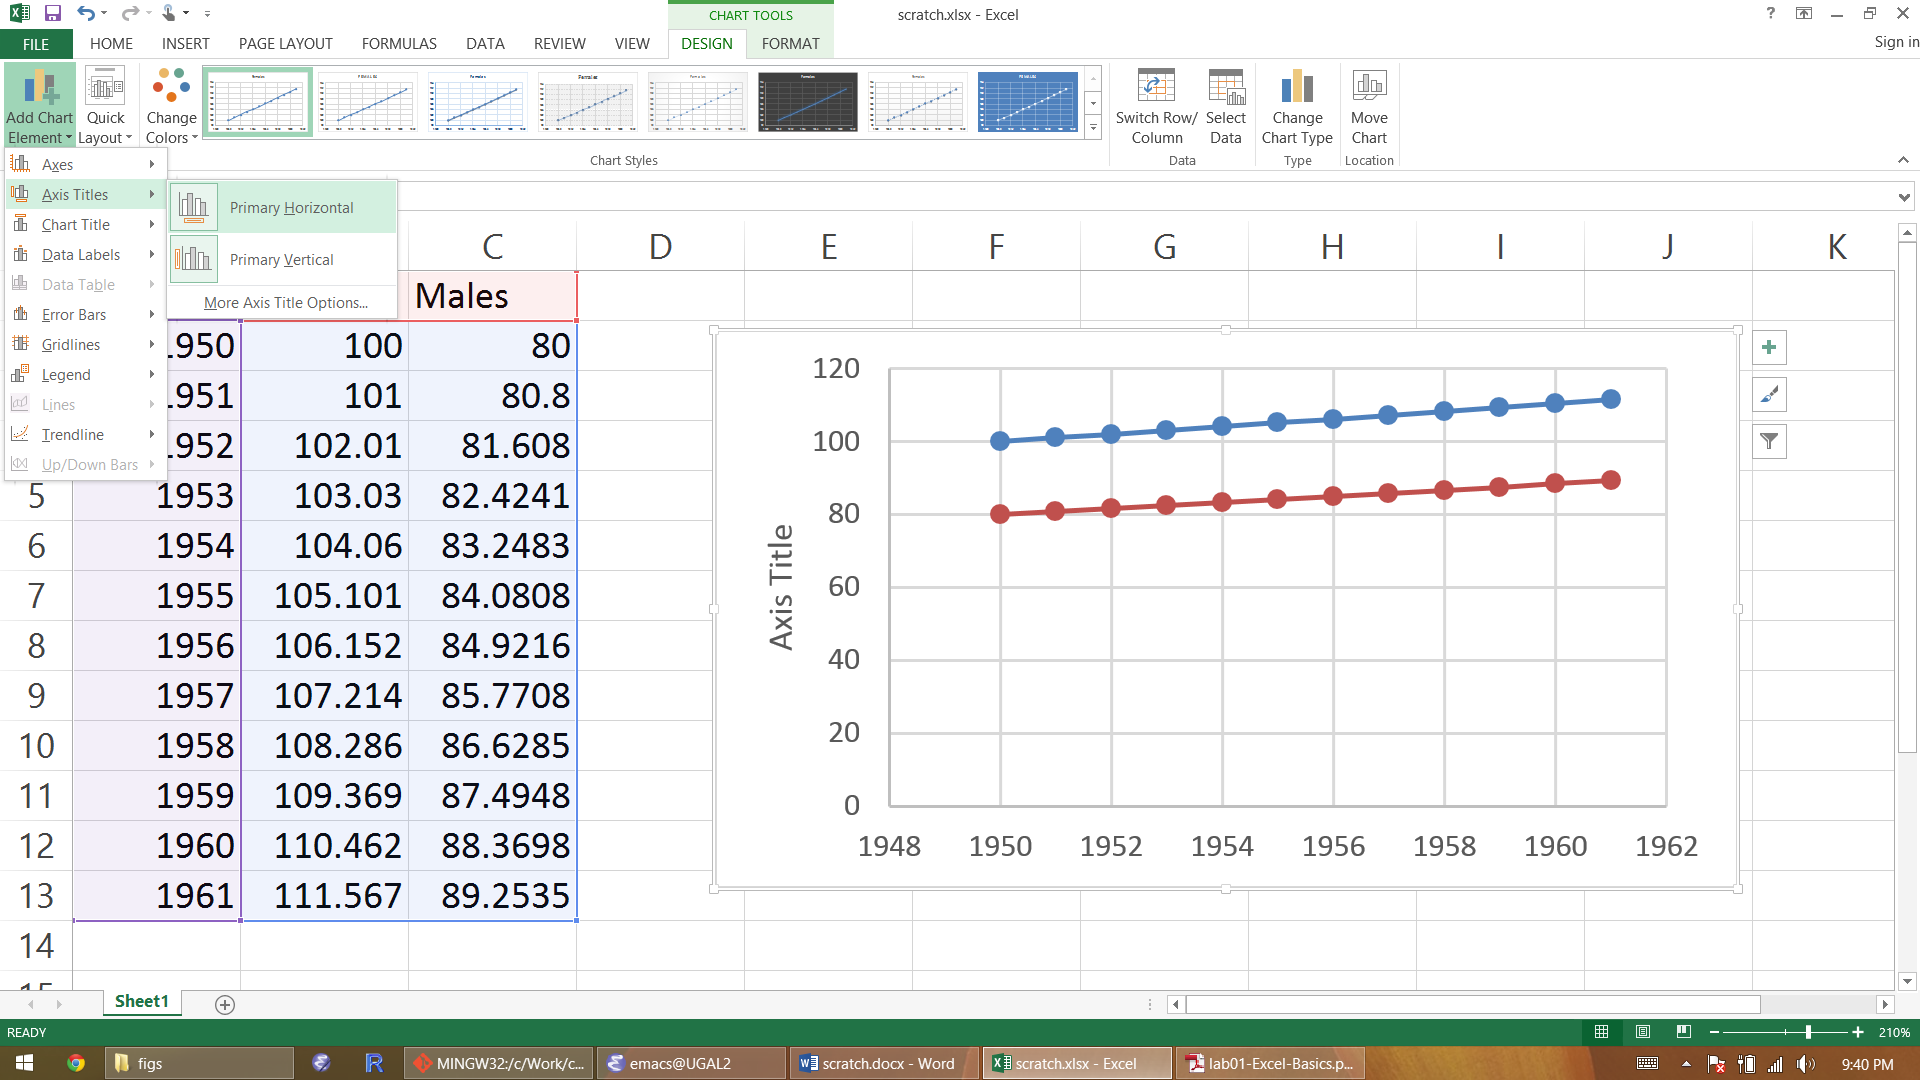
\includegraphics[width=\textwidth]{figs/customize2}}}
%  \end{overprint}
    \begin{center}
      Add legend
    \end{center}
\end{frame}



\begin{frame}
  \frametitle{Customize}
    \fbox{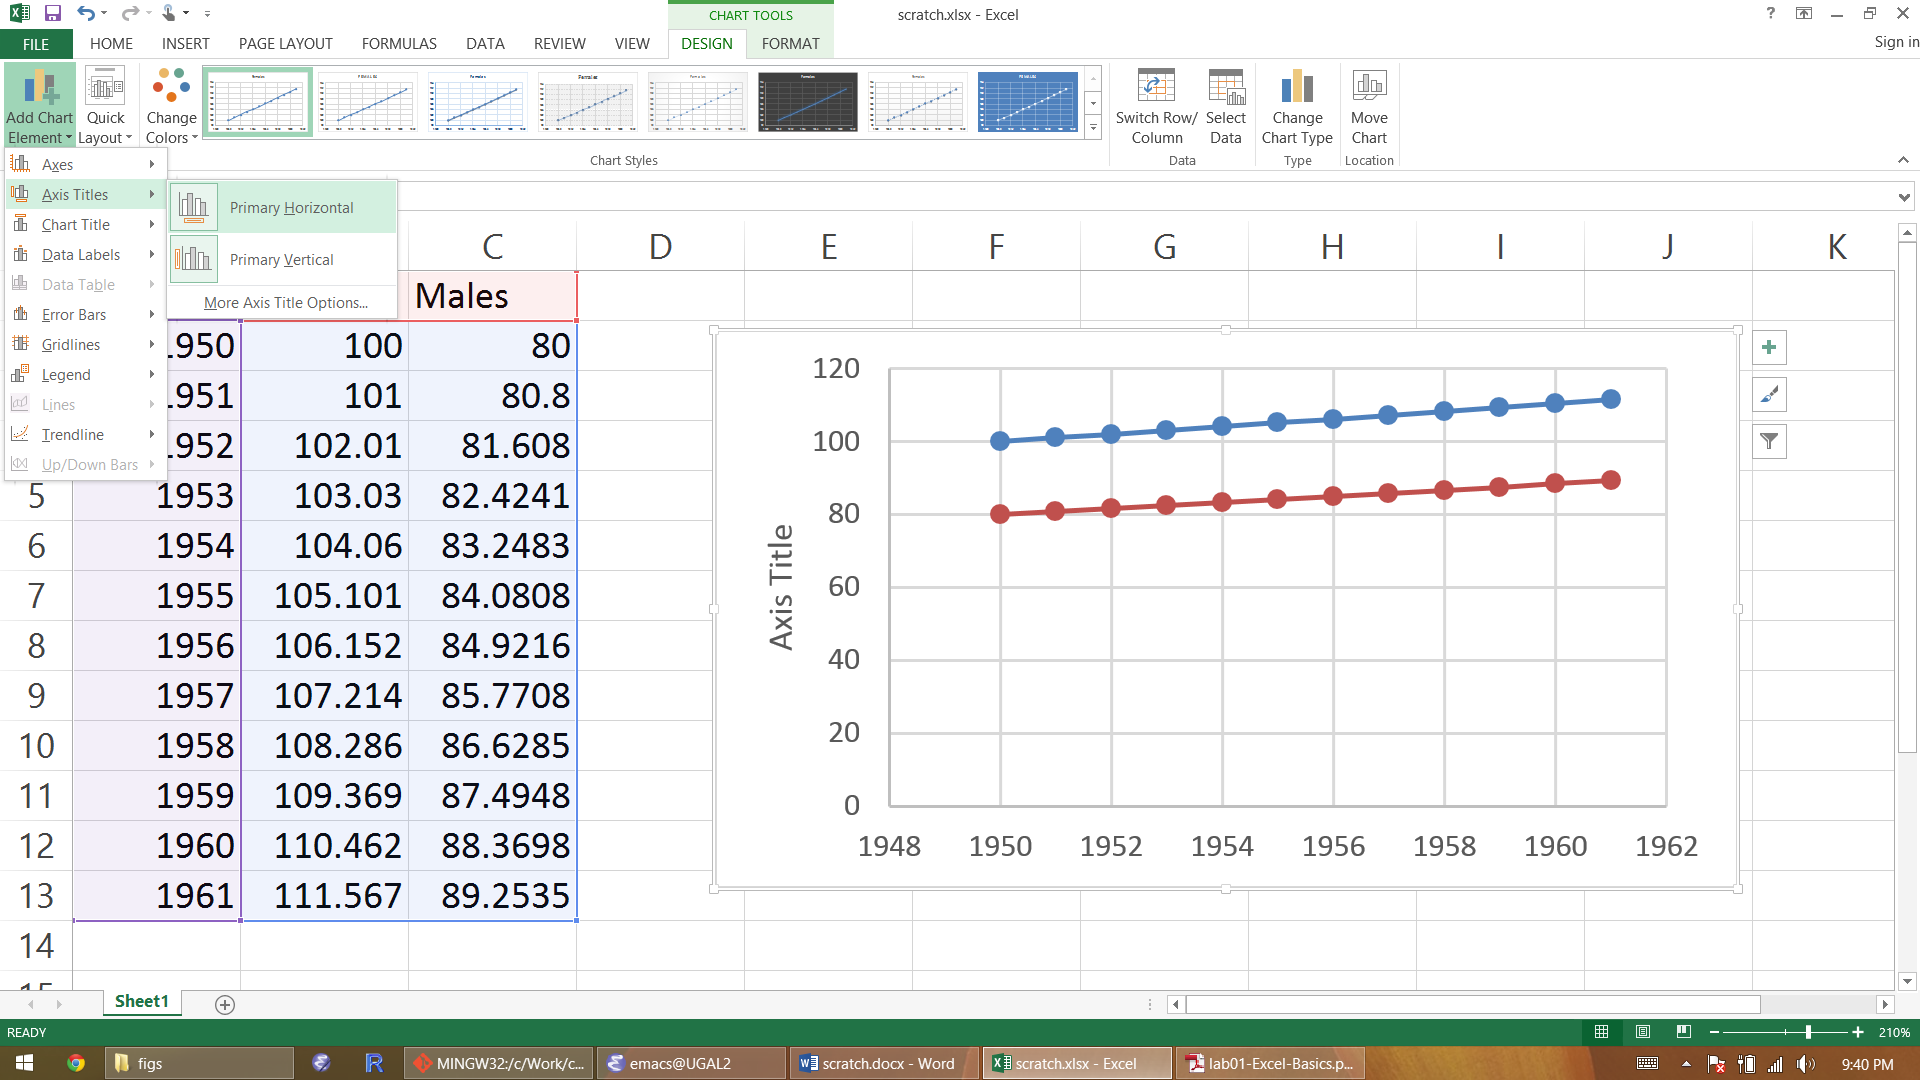
\includegraphics[width=\textwidth]{figs/customize2}}
    \begin{center}
      Add axis labels
    \end{center}
\end{frame}



\begin{frame}
  \frametitle{Customize}
    \fbox{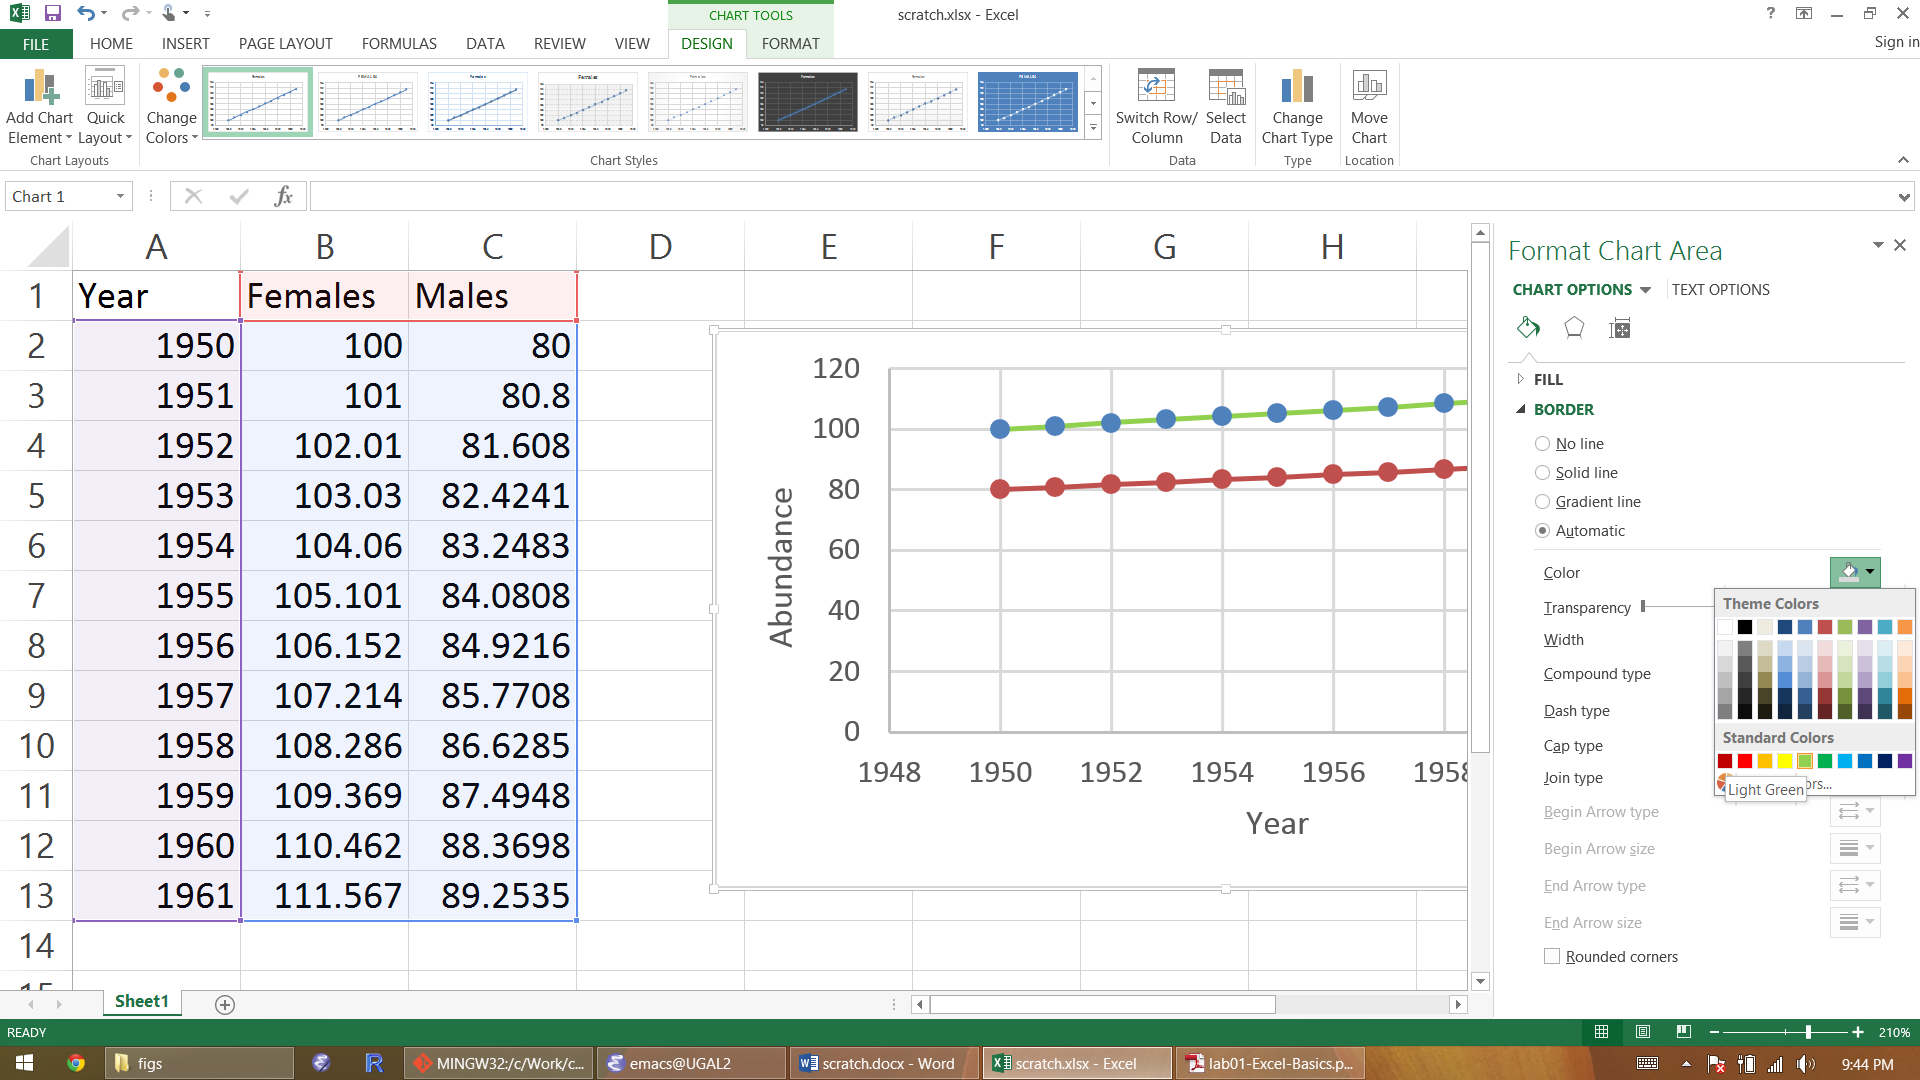
\includegraphics[width=\textwidth]{figs/customize3}}
    \begin{center}
      Change line color
    \end{center}
\end{frame}



% \section{In-class exercise}



% \begin{frame}
%   \frametitle{In-class exercise}
%   \fbox{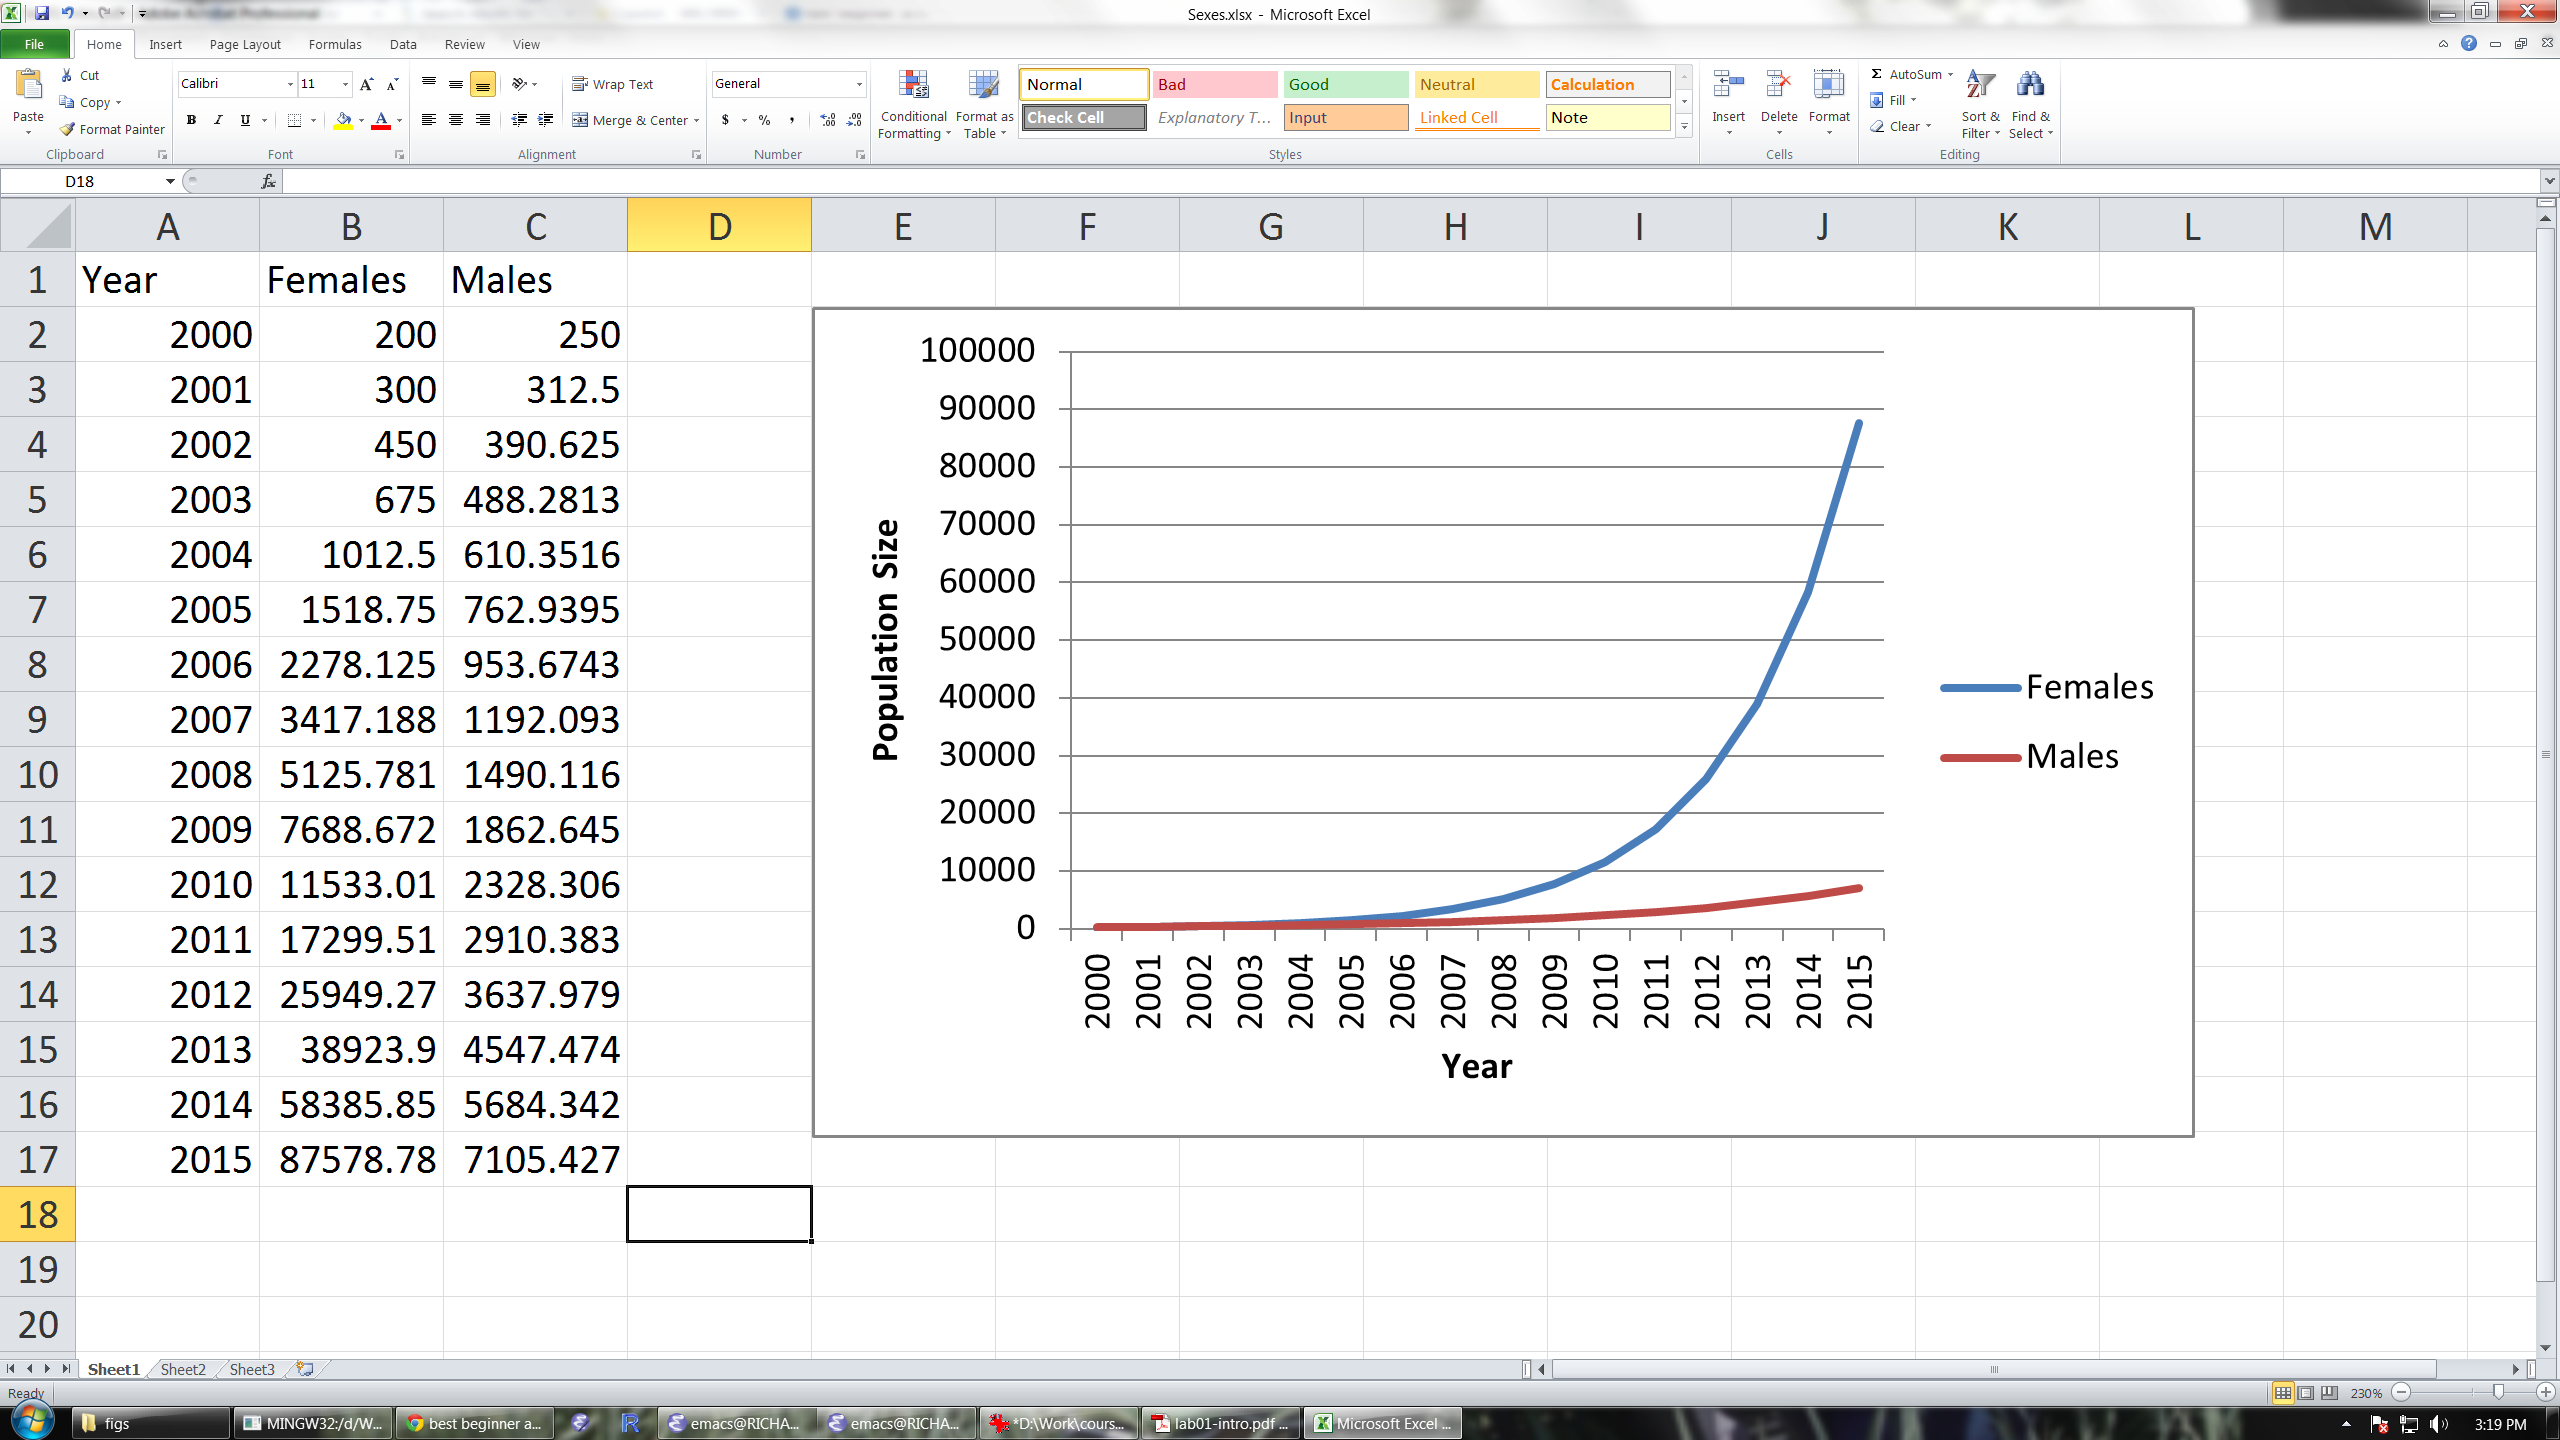
\includegraphics[width=\textwidth]{figs/inclass1}}
% \end{frame}




% \section{Assignment}


% \begin{frame}
%   \frametitle{Assignment}
%   \small
%   \begin{enumerate}[(1)]
%     \item Create an Excel file and name it
%       ``Yourlastname-yourfirstname''
%     \item Create the sheet shown below using techniques covered in
%       this lab (don't just type the numbers in)
%     \item Upload to ELC Dropbox (\url{elcnew.uga.edu})
%   \end{enumerate}
%   \begin{center}
%     \fbox{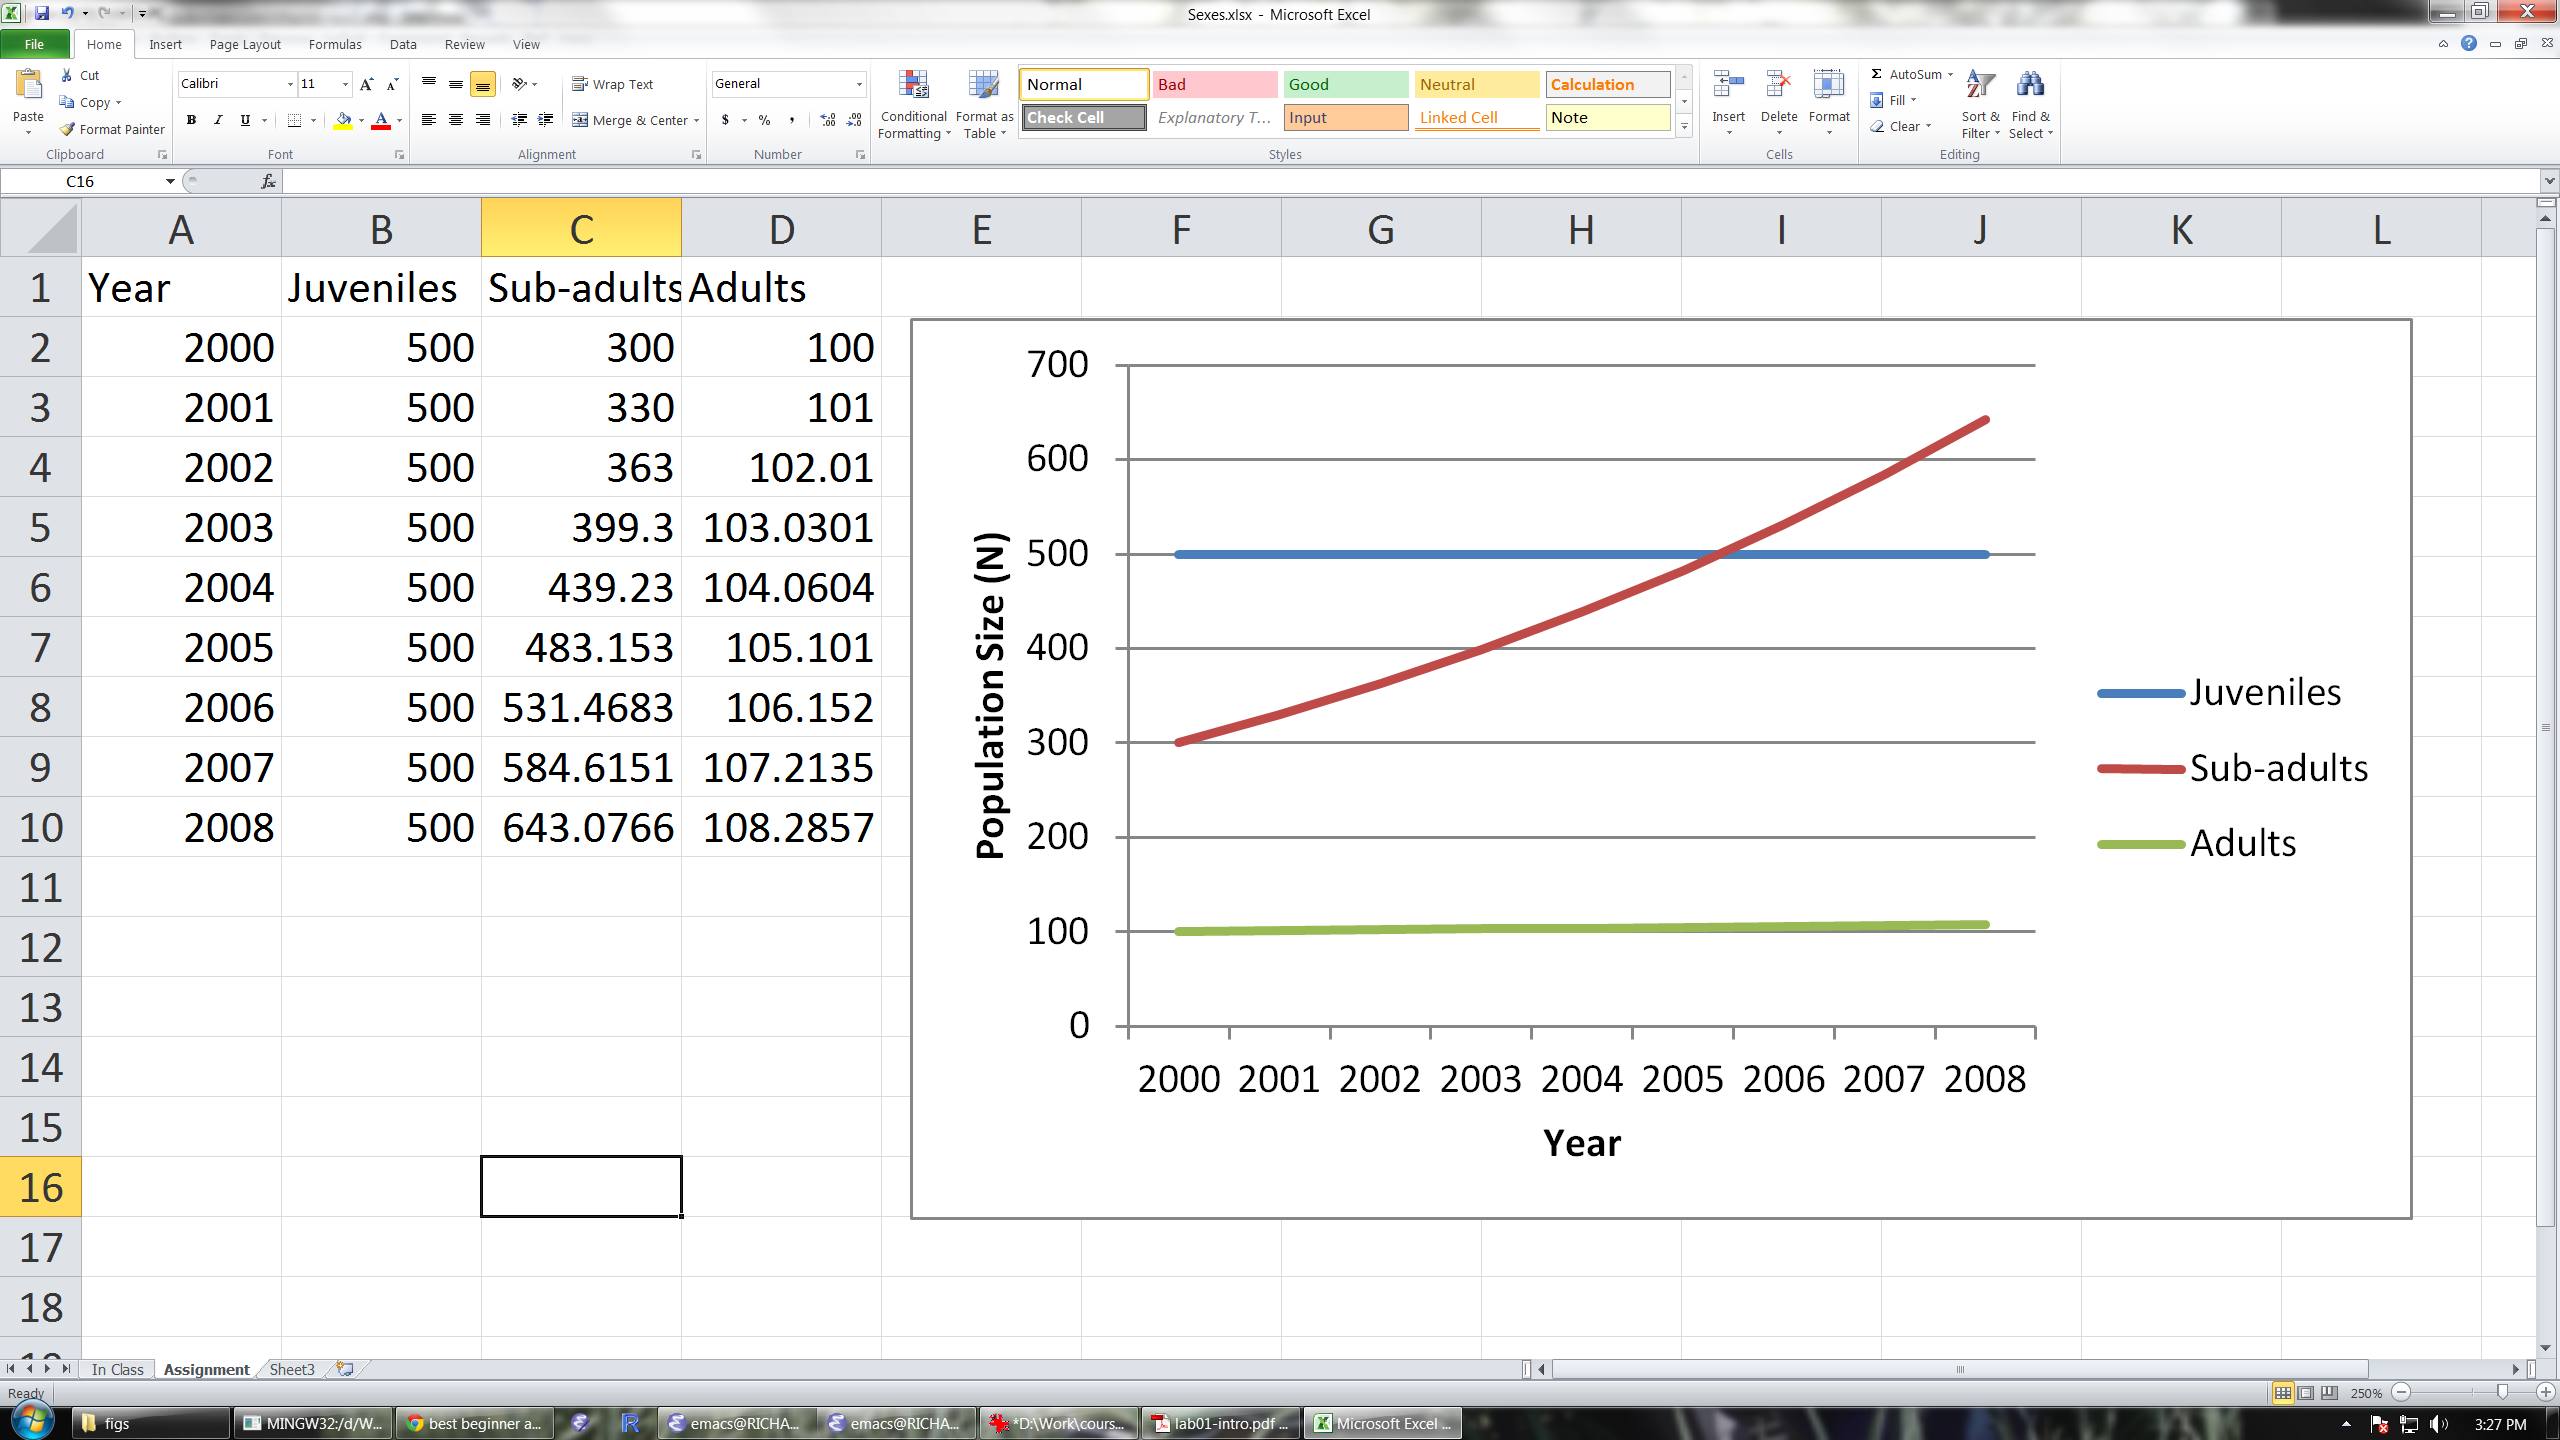
\includegraphics[width=0.7\textwidth]{figs/assignment}}
%   \end{center}
% \end{frame}



\end{document}
